\documentclass[aspectratio=169, lualatex, handout]{beamer}
\makeatletter\def\input@path{{theme/}}\makeatother\usetheme{cipher}

\title{Applied Cryptography}
\author{Nadim Kobeissi}
\institute{American University of Beirut}
\instituteimage{images/aub_white.png}
\date{\today}
\coversubtitle{CMPS 297AD/396AI\\Fall 2025}
\coverpartname{Part 2: Real-World Cryptography}
\covertopicname{2.4: End-to-End Encrypted Cloud Storage}
\coverwebsite{https://appliedcryptography.page}

\begin{document}
\begin{frame}[plain]
	\titlepage
\end{frame}

\section{Introduction}

\begin{frame}{Cloud storage today}
	\begin{columns}[c]
		\begin{column}{0.5\textwidth}
			\begin{itemize}
				\item Cloud storage is a prevalent computing paradigm today
				\item Outsources data storage to third party services
				\item Benefits for users:
				      \begin{itemize}
					      \item No need to worry about backups
					      \item High data availability
					      \item Access data from anywhere
				      \end{itemize}
				\item Major providers (Google, Microsoft, Apple, Amazon) control encryption keys
			\end{itemize}
		\end{column}
		\begin{column}{0.5\textwidth}
			\imagewithcaption{onedrive.png}{Microsoft OneDrive is an example of a popular cloud storage service.}
		\end{column}
	\end{columns}
\end{frame}

\begin{frame}{Regular vs End-to-End Encrypted Cloud Storage}
	\begin{columns}
		\begin{column}{0.5\textwidth}
			\textbf{Regular Cloud Storage}\\
			\textit{(e.g., OneDrive, Google Drive)}
			\vspace{0.5cm}
			\begin{itemize}
				\item \textbf{Transport encryption:} TLS protects data in transit
				\item \textbf{Encryption at rest:} Provider encrypts on their servers
				\item \textbf{Provider controls keys:} Can decrypt your data
			\end{itemize}
		\end{column}
		\begin{column}{0.5\textwidth}
			\textbf{E2E Encrypted Storage}\\
			\textit{(e.g., MEGA, Nextcloud)}
			\vspace{0.5cm}
			\begin{itemize}
				\item \textbf{Client-side encryption:} Data encrypted before upload
				\item \textbf{User controls keys:} Provider never sees plaintext
				\item \textbf{Confidentiality:} Provider learns nothing about content
			\end{itemize}
		\end{column}
	\end{columns}
\end{frame}

\begin{frame}{Regular vs End-to-End Encrypted Cloud Storage}
	\begin{columns}
		\begin{column}{0.5\textwidth}
			\textbf{Regular Cloud Storage}\\
			\textit{(e.g., OneDrive, Google Drive)}
			\\
			\vspace{0.5cm}
			\textbf{Risks:}
			\begin{itemize}
				\item Provider breach exposes data
				\item Government requests
				\item Insider threats
				\item Provider can analyze content
			\end{itemize}
		\end{column}
		\begin{column}{0.5\textwidth}
			\textbf{E2E Encrypted Storage}\\
			\textit{(e.g., MEGA, Nextcloud)}
			\\
			\vspace{0.5cm}
			\textbf{Guarantees:}
			\begin{itemize}
				\item Provider breach reveals nothing
				\item Government gets encrypted data
				\item No insider access to content
				\item Provider can only analyze metadata
			\end{itemize}
		\end{column}
	\end{columns}
\end{frame}

\begin{frame}{End-to-End Encryption (E2EE) for cloud storage}
	\begin{itemize}
		\item Alternative approach: Users encrypt before uploading
		\item Users control their own encryption keys
		\item Security guarantees:
		      \begin{itemize}
			      \item Cryptographic confidentiality
			      \item Authenticity and integrity protection
			      \item Provider can't read file contents
			      \item Provider can't modify files undetectably
		      \end{itemize}
		\item Security maintained even if service is compromised
		\item Ideally secure against malicious service providers
	\end{itemize}
\end{frame}

\begin{frame}{Key management challenges}
	\begin{itemize}
		\item Key management delegated to users
		\item Humans are poor at memorizing cryptographic keys
		\item Security typically bootstrapped from passwords
		\item Fundamental limitation: Dictionary attacks possible
		\item Trade-off between convenience and security
		\item Strong password policies can partially mitigate risks
	\end{itemize}
\end{frame}

\begin{frame}{Password hashing}
	\begin{columns}[c]
		\begin{column}{1\textwidth}
			\begin{itemize}
				\item Users typically access E2EE storage via passwords
				\item Passwords must be converted to cryptographic keys
				\item Common approach: password hashing\footnote{This was previously covered in our \textit{Collision-Resistant Hash Functions} topic.}
				\item Popular password hashing functions:
				      \begin{itemize}
					      \item \textbf{PBKDF2}: Widely deployed but aging
					      \item \textbf{scrypt}: Memory-hard against ASICs
					      \item \textbf{Argon2}: Winner of Password Hashing Competition
				      \end{itemize}
				\item KDFs slow down brute-force attacks
				\item Still vulnerable to dictionary attacks with weak passwords
			\end{itemize}
		\end{column}
	\end{columns}
\end{frame}

\begin{frame}{The authentication vs encryption dilemma}
	\begin{columns}[c]
		\begin{column}{1\textwidth}
			\begin{itemize}
				\item Traditional services: Server stores password hash
				\item E2EE requirement: Server must never see encryption key
				\item Two common approaches:
				      \begin{itemize}
					      \item \textbf{Dual-password:} Separate login and encryption passwords
					      \item \textbf{SRP (Secure Remote Password):} Zero-knowledge proof of password
					      \item \textbf{Hardware-backed authentication:} Passkeys, Apple Secure Enclave, etc.
				      \end{itemize}
				\item Trade-offs:
				      \begin{itemize}
					      \item Dual-password: Poor usability, users often reuse
					      \item SRP: Complex implementation
					      \item Hardware-backed: Requires specific devices/platforms
				      \end{itemize}
				\item MEGA uses custom authentication with encryption keys
			\end{itemize}
		\end{column}
	\end{columns}
\end{frame}

\begin{frame}{Password recovery challenges}
	\begin{itemize}
		\item Lost password = lost data in true E2EE
		      \begin{itemize}
			      \item The ``mud puddle test''
		      \end{itemize}
		\item Users expect password recovery options
		\item Common mitigation strategies:
		      \begin{itemize}
			      \item \textbf{Recovery keys:} Long random string users must store
			      \item \textbf{Social recovery:} Threshold sharing among contacts
			      \item \textbf{Security questions:} Weaker but familiar to users
		      \end{itemize}
	\end{itemize}
\end{frame}

\begin{frame}{Apple's Advanced Data Protection}
	\begin{columns}[c]
		\begin{column}{1\textwidth}
			\begin{itemize}
				\item Apple introduced optional E2EE for iCloud in 2023\footnote{\url{https://support.apple.com/en-us/102651}}
				\item Called ``Advanced Data Protection'' (ADP)
				\item Covers most iCloud data categories:
				      \begin{itemize}
					      \item Photos, Notes, iCloud Backup, Messages backup
					      \item iCloud Drive, Reminders, Safari bookmarks
				      \end{itemize}
				\item Apple's approach to recovery:
				      \begin{itemize}
					      \item \textbf{Option 1:} User-managed recovery key
					      \item \textbf{Option 2:} Apple escrow (default)
					      \item Users must explicitly opt-in to ADP
				      \end{itemize}
				\item Fundamental tension: Security vs recoverability
				\item Apple chose user choice over mandatory E2EE
			\end{itemize}
		\end{column}
	\end{columns}
\end{frame}

\begin{frame}{Multi-device key management}
	\begin{itemize}
		\item Users expect seamless multi-device access
		\item Each device needs access to encryption keys
		\item Key synchronization approaches:
		      \begin{itemize}
			      \item \textbf{Password-based:} Derive keys on each device
			      \item \textbf{Device pairing:} Transfer keys device-to-device
			      \item \textbf{Cloud keychain:} Encrypted key storage (circular problem)
		      \end{itemize}
		\item Additional challenges:
		      \begin{itemize}
			      \item Device revocation when lost/stolen
			      \item Key rotation after compromise
			      \item Offline device synchronization
		      \end{itemize}
	\end{itemize}
\end{frame}

\begin{frame}{Research directions in usable key management}
	\begin{itemize}
		\item \textbf{Threshold cryptography:} Split keys across multiple locations
		\item \textbf{Hardware tokens:} FIDO2/WebAuthn/Passkeys for encryption key storage
		\item \textbf{Biometric key derivation:} Fuzzy extractors from fingerprints
		\item \textbf{Social key recovery:} Friends/family as key custodians
		\item Open problems:
		      \begin{itemize}
			      \item Balancing security with grandmother-friendliness
			      \item Recovery without trusted third parties
			      \item Protecting against coercion/rubber-hose attacks
		      \end{itemize}
		\item Most solutions add complexity or trust assumptions
	\end{itemize}
\end{frame}

\begin{frame}{Passkeys: A new authentication paradigm}{Quick aside}
	\begin{columns}[c]
		\begin{column}{0.6\textwidth}
			\begin{itemize}
				\item \textbf{Passkeys} are a password replacement based on WebAuthn/FIDO2
				\item Built on public-key cryptography:
				      \begin{itemize}
					      \item Private key stored securely on device
					      \item Public key registered with service
					      \item Authentication via cryptographic signatures
				      \end{itemize}
				\item Key advantages over passwords:
				      \begin{itemize}
					      \item Phishing-resistant by design
					      \item No shared secrets with server
					      \item Automatic strong credentials
				      \end{itemize}
				\item Apple: iCloud Keychain, Microsoft: Windows Hello\ldots
			\end{itemize}
		\end{column}
		\begin{column}{0.4\textwidth}
			\imagewithcaption{passkeys_mac.png}{Passkey dialog on macOS.}
		\end{column}
	\end{columns}
\end{frame}

\begin{frame}{WebAuthn PRF: symmetric keys from passkeys}{Quick aside}
	\begin{itemize}
		\item WebAuthn's \textbf{PRF (Pseudo-Random Function)} extension enables key derivation
		\item Key derivation process:
		      \begin{itemize}
			      \item PRF can be evaluated during credential creation/assertion
			      \item Produces 32-byte outputs suitable for encryption keys
			      \item Supports two inputs per operation (for key rotation)
		      \end{itemize}
		\item Implementation typically uses HMAC-SHA256 internally
	\end{itemize}
\end{frame}

\begin{frame}{$\mathsf{PRF}: F_{k}= X \rightarrow Y$}{Reminder}
	\begin{columns}[c]
		\begin{column}{0.4\textwidth}
			\begin{itemize}
				\item We want the mapping to be:
				      \begin{itemize}
					      \item One-way
					      \item ``Randomized''
					      \item Relations between inputs not reflected in outputs
				      \end{itemize}
			\end{itemize}
		\end{column}

		\begin{column}{0.8\textwidth}
			\begin{tikzpicture}[scale=0.38]
				% Define colors
				\definecolor{domaingreen}{RGB}{102, 170, 68}
				\definecolor{rangegreen}{RGB}{170, 187, 136}
				\definecolor{circlecolor}{RGB}{235, 137, 85}
				\definecolor{purplearrow}{RGB}{160, 78, 160}
				\definecolor{redarrow}{RGB}{237, 50, 36}

				% Input space (domain) X - made square
				\draw[dashed, thick, domaingreen, fill=domaingreen]
				(0,0) rectangle (8,8);
				\node[text width=6.5cm, align=center, font=\normalsize]
				at
				(4,-0.8)
				{Size: infinite!};
				\node[font=\small] at (4,9) {Input space (domain) $X$};

				% Output (range) Y - made square - moved more to the right
				\draw[thick, rangegreen, fill=rangegreen] (15,2) rectangle (20,7);
				\node[text width=4cm, align=center, font=\normalsize]
				at
				(17.5,1.2)
				{Size: fixed};
				\node[font=\small] at (17.5,8.5) {Output (range) $Y$};
				% Input dots - adjusted positions for square domain
				\filldraw[circlecolor] (2,7) circle (0.3);
				\pause
				\draw[-{Stealth[length=6mm, width=4mm]}, thick, purplearrow]
				(2,7) -- (16.2,6.4);
				\pause
				\filldraw[circlecolor] (16.2,6.4) circle (0.3);
				\pause

				\filldraw[circlecolor] (3,6) circle (0.3);
				\pause
				\draw[-{Stealth[length=6mm, width=4mm]}, thick, purplearrow]
				(3,6) -- (18.6,5.3);
				\pause
				\filldraw[circlecolor] (18.6,5.3) circle (0.3);
				\pause

				\filldraw[circlecolor] (2,5) circle (0.3);
				\pause
				\draw[-{Stealth[length=6mm, width=4mm]}, thick, purplearrow]
				(2,5) -- (16.8,4.2);
				\pause
				\filldraw[circlecolor] (16.8,4.2) circle (0.3);
				\pause

				\filldraw[circlecolor] (4,3.5) circle (0.3);
				\pause
				\draw[-{Stealth[length=6mm, width=4mm]}, thick, purplearrow]
				(4,3.5) -- (18.4,3.2);
				\pause
				\filldraw[circlecolor] (18.4,3.2) circle (0.3);
				\pause

				\filldraw[circlecolor] (2,2) circle (0.3);
				\pause
				\draw[-{Stealth[length=6mm, width=4mm]}, thick, purplearrow]
				(2,2) -- (17.1,2.7);
				\pause
				\filldraw[circlecolor] (17.1,2.7) circle (0.3);
				\pause

				\filldraw[circlecolor] (3,1) circle (0.3);
				\pause
				\draw[-{Stealth[length=6mm, width=4mm]}, ultra thick, redarrow]
				(3,1) -- (16.8,4.2);
				\node[redarrow, font=\scriptsize\bfseries, rotate=14]
				at
				(10,3)
				{Collisions are inevitable};
			\end{tikzpicture}
		\end{column}
	\end{columns}
\end{frame}

\begin{frame}{Using passkeys for key management}{Quick aside}
	\begin{itemize}
		\item Potential architecture combining passkeys with E2EE:
		      \begin{itemize}
			      \item User authenticates with passkey (no password needed)
			      \item PRF extension derives encryption keys on-demand
			      \item Keys never leave the authenticator/device
		      \end{itemize}
		\item Benefits:
		      \begin{itemize}
			      \item No password-derived keys (stronger security)
			      \item Hardware-backed key storage
			      \item Seamless multi-device via platform sync
		      \end{itemize}
		\item Current limitations:
		      \begin{itemize}
			      \item PRF extension not universally supported
			      \item Security keys may not support PRF evaluation at creation
		      \end{itemize}
		\item Represents potential future direction for usable E2EE key management and authentication more generally
	\end{itemize}
\end{frame}

\begin{frame}{File sharing challenges}
	\begin{itemize}
		\item Primary feature: Sharing files with selected users
		\item Recipients need decryption keys
		\item Keys cannot be sent unprotected via untrusted provider
		\item Common solutions:
		      \begin{itemize}
			      \item Encrypt file key under recipient's public key
			      \item Use out-of-band mechanisms
		      \end{itemize}
	\end{itemize}
\end{frame}

\begin{frame}{E2EE cloud storage providers}
	\begin{itemize}
		\item Major providers:
		      \begin{itemize}
			      \item MEGA: 300M users, 150B files, 1000 PB data
			      \item Nextcloud
			      \item Apple iCloud (optional E2EE since 2023)
		      \end{itemize}
		\item Smaller providers:
		      \begin{itemize}
			      \item icedrive, pCloud, Seafile, Tresorit
			      \item Tens of millions of users collectively
		      \end{itemize}
	\end{itemize}
\end{frame}

\begin{frame}{Security concerns with current E2EE providers}
	\begin{itemize}
		\item Recent analyses found attacks on MEGA and Nextcloud
		\item Both providers use complex, ad hoc cryptographic designs
		\item Lack formal security guarantees
		\item MEGA's challenges:
		      \begin{itemize}
			      \item Migration infeasible - requires user participation
			      \item Initial minimal patches proved insufficient
			      \item Required second round of complex patching
		      \end{itemize}
		\item Nextcloud's response:
		      \begin{itemize}
			      \item Forced to disable E2EE file sharing entirely
			      \item Significant feature regression
			      \item Required full redesign
		      \end{itemize}
	\end{itemize}
\end{frame}

\begin{frame}{Current state of E2EE Cloud Storage}
	\begin{itemize}
		\item Most providers rely on proprietary, unanalyzed designs
		\item Highlights need for formally analyzed cryptographic designs
		\item Security confidence lags behind E2EE messaging and browsing
		\item Less design input from cryptographic research community
		\item Need for standardized, proven security approaches
		\item \textbf{In this topic, we'll cover:} \begin{enumerate}
			      \item What went wrong with MEGA
			      \item What went wrong with Nextcloud
			      \item A quick look at WhatsApp encrypted cloud backups
			      \item An attempt by cryptographers to design a provably secure E2EE Cloud Storage protocol
		      \end{enumerate}
	\end{itemize}
\end{frame}

\section{Attacks on MEGA and Nextcloud}

\subsection{Attacks on MEGA}

\begin{frame}{MEGA: Overview}
	\begin{columns}[c]
		\begin{column}{0.75\textwidth}
			\begin{itemize}
				\item Founded in 2013 by Kim Dotcom (post-Megaupload)
				\item One of the largest E2EE cloud storage providers
				\item \textbf{Key statistics}:
				      \begin{itemize}
					      \item Over 300 million registered users\footnote{\url{https://blog.mega.io/mega-reaches-300-million-users-milestone}}
					      \item 150+ billion files stored
				      \end{itemize}
				\item \textbf{Core features}:
				      \begin{itemize}
					      \item Client-side encryption before upload
					      \item Secure file sharing via encrypted links
					      \item Cross-platform support (web, desktop, mobile)
					      \item Free tier with 20 GB storage
				      \end{itemize}
				\item All encryption performed in JavaScript (web client)
			\end{itemize}
		\end{column}
		\begin{column}{0.25\textwidth}
			\imagewithcaption{mega_logo.png}{MEGA's logo.}
		\end{column}
	\end{columns}
\end{frame}

\begin{frame}{MEGA: Key hierarchy}
	\begin{columns}[c]
		\begin{column}{0.6\textwidth}
			\begin{itemize}
				\item Password serves as root of trust for entire key hierarchy
				\item Key derivation from password:
				      \begin{itemize}
					      \item \textbf{Authentication key:} Identifies user to MEGA
					      \item \textbf{Encryption key:} Encrypts the master key
				      \end{itemize}
				\item \textbf{Master key:} Randomly generated, encrypts all other keys
			\end{itemize}
		\end{column}
		\begin{column}{0.4\textwidth}
			\imagewithcaption{mega_keys.png}{MEGA's key hierarchy. The master key encrypts the share, chat, sign
				and node keys using AES-ECB. Source: \url{https://appliedcryptography.page/papers/\#mega-awry}}
		\end{column}
	\end{columns}
\end{frame}

\begin{frame}{MEGA: Key hierarchy}
	\begin{columns}[c]
		\begin{column}{0.6\textwidth}
			\begin{itemize}
				\item Asymmetric key pairs for each account:
				      \begin{itemize}
					      \item \textbf{RSA key pair:} For data sharing
					      \item \textbf{Curve25519 key pair:} For chat key exchange
					      \item \textbf{Ed25519 key pair:} For signing other keys
				      \end{itemize}
				\item \textbf{Per-node keys:} New key for each file/folder
				\item All keys encrypted with master key using AES-ECB
				\item Encrypted keys stored on MEGA servers
				\item Enables multi-device access with password only
			\end{itemize}
		\end{column}
		\begin{column}{0.4\textwidth}
			\imagewithcaption{mega_keys.png}{MEGA's key hierarchy. The master key encrypts the share, chat, sign
				and node keys using AES-ECB. Source: \url{https://appliedcryptography.page/papers/\#mega-awry}}
		\end{column}
	\end{columns}
\end{frame}

\begin{frame}{MEGA: Where's the attack?}
	\bigimagewithcaption{mega_keys.png}{MEGA's key hierarchy. The master key encrypts the share, chat, sign
		and node keys using AES-ECB. Source: \url{https://appliedcryptography.page/papers/\#mega-awry}}
\end{frame}

\begin{frame}{MEGA: Key hierarchy}
	\begin{columns}[c]
		\begin{column}{1\textwidth}
			\begin{itemize}
				\item Password-to-key derivation
				\item MEGA uses HKDF for deriving keys from password
				\item \textbf{Problem:} HKDF is not a password hash!
				      \begin{itemize}
					      \item HKDF designed for key derivation from high-entropy inputs
					      \item No computational hardness against brute-force
					      \item Passwords have low entropy
				      \end{itemize}
				\item \textbf{Should use:} Argon2, scrypt, or PBKDF2
				      \begin{itemize}
					      \item Memory-hard functions
					      \item Configurable iteration counts
					      \item Resistance to GPU/ASIC attacks
				      \end{itemize}
				\item Enables offline dictionary attacks on user passwords
			\end{itemize}
		\end{column}
	\end{columns}
\end{frame}

\begin{frame}{Attack 1: RSA key recovery attack}
	\begin{columns}[c]
		\begin{column}{0.6\textwidth}
			\begin{itemize}
				\item \textbf{Target:} User's RSA private key (for sharing)
				\item \textbf{Exploit:} No integrity protection on encrypted RSA key
				\item \textbf{Attack vector:}
				      \begin{itemize}
					      \item Malicious server modifies encrypted RSA key
					      \item Client decrypts corrupted key
					      \item RSA-CRT implementation leaks information
				      \end{itemize}
				\item \textbf{Oracle construction:}
				      \begin{itemize}
					      \item Each login attempt leaks 1 bit
					      \item About RSA modulus factors
				      \end{itemize}
			\end{itemize}
		\end{column}
		\begin{column}{0.4\textwidth}
			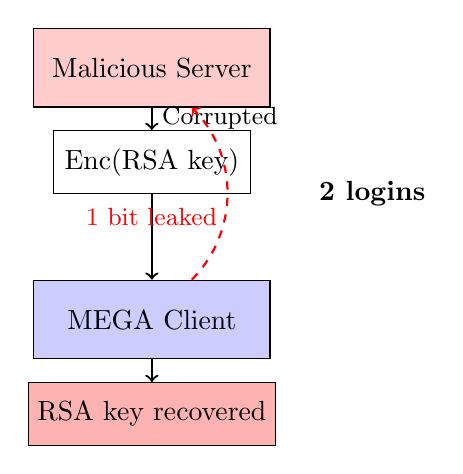
\begin{tikzpicture}[scale=0.8]
				% Server
				\node[draw, rectangle, minimum width=3cm, minimum height=1cm, fill=red!20] (server) at (0,4) {Malicious Server};

				% Client
				\node[draw, rectangle, minimum width=3cm, minimum height=1cm, fill=blue!20] (client) at (0,0) {MEGA Client};

				% Encrypted RSA key
				\node[draw, rectangle, minimum width=2.5cm, minimum height=0.8cm] (enckey) at (0,2.5) {Enc(RSA key)};

				% Attack flow
				\draw[->, thick] (server) -- node[right] {\small Corrupted} (enckey);
				\draw[->, thick] (enckey) -- (client);

				% Oracle feedback
				\draw[->, thick, dashed, red] (client) to[bend right=45] node[left, yshift=-0.3cm] {\small 1 bit leaked} (server);

				% Result
				\node[draw, rectangle, minimum width=3cm, minimum height=0.8cm, fill=red!30] (result) at (0,-1.5) {RSA key recovered};
				\draw[->, thick] (client) -- (result);

				% Attack count
				\node at (3.5,2) {\textbf{2 logins}};
			\end{tikzpicture}
		\end{column}
	\end{columns}
\end{frame}

\begin{frame}{Attack 1: High-level overview}
	\begin{columns}[c]
		\begin{column}{1\textwidth}
			\begin{itemize}
				\item \textbf{Threat model:} Malicious service provider controls MEGA infrastructure
				\item \textbf{Attack strategy:}
				      \begin{enumerate}
					      \item Modify encrypted RSA private key (no integrity protection)
					      \item Use modified key to create decryption oracle
					      \item Binary search to recover RSA prime factor
				      \end{enumerate}
				\item \textbf{Key insight:} RSA-CRT implementation leaks information
				      \begin{itemize}
					      \item Modified key causes different behavior for $m < q$ vs $m \geq q$
					      \item Where $q$ is one of the RSA primes
					      \item Observable through session ID responses
				      \end{itemize}
				\item \textbf{Attack efficiency:}
				      \begin{itemize}
					      \item Binary search requires ~512 login attempts\footnote{Later improved to 2 logins: \url{https://appliedcryptography.page/papers/\#mega-recovery}}
					      \item Each login leaks 1 bit of information about $q$
				      \end{itemize}
			\end{itemize}
		\end{column}
	\end{columns}
\end{frame}

\begin{frame}{Attack 1: The decryption oracle}
	\begin{columns}[c]
		\begin{column}{0.5\textwidth}
			\begin{itemize}
				\item \textbf{Setup:}
				      \begin{itemize}
					      \item Server sends corrupted RSA key
					      \item Key has modified $u' \neq u = q^{-1} \bmod p$
				      \end{itemize}
				\item \textbf{Oracle mechanism:}
				      \begin{itemize}
					      \item Server chooses message $m$
					      \item Sends encrypted $[m]_{pk}$ as session ID
					      \item Client decrypts with corrupted key
				      \end{itemize}
				\item \textbf{Observable behavior:}
				      \begin{itemize}
					      \item If $m < q$: Returns $\text{sid}' = 0$
					      \item If $m \geq q$: Returns $\text{sid}' \neq 0$
				      \end{itemize}
			\end{itemize}
		\end{column}
		\begin{column}{0.5\textwidth}
			\begin{tikzpicture}[scale=0.8]
				% Binary search visualization
				\node[draw, rectangle, minimum width=4cm, minimum height=0.5cm] (range) at (0,3) {Search range for $q$};

				% Middle point
				\node[draw, circle, fill=yellow!30] (mid) at (0,2) {$m$};
				\draw[->, thick] (range) -- (mid);

				% Oracle
				\node[draw, rectangle, minimum width=3cm, minimum height=0.8cm, fill=blue!20] (oracle) at (0,0.5) {Decryption Oracle};
				\draw[->, thick] (mid) -- (oracle);

				% Decision
				\node[draw, diamond, aspect=2, fill=green!20] (decision) at (0,-1.5) {$m < q?$};
				\draw[->, thick] (oracle) -- (decision);

				% Left and right
				\node at (-2,-3) {Left half};
				\node at (2,-3) {Right half};
				\draw[->, thick] (decision) -- (-2,-2.5) node[midway, left, xshift=-3mm] {Yes};
				\draw[->, thick] (decision) -- (2,-2.5) node[midway, right, xshift=3mm] {No};

				% Iteration count
				\node[draw, rectangle, fill=red!20] at (4.5,0) {2 iterations};
			\end{tikzpicture}
		\end{column}
	\end{columns}
\end{frame}

\begin{frame}{Attack 2: Plaintext recovery attack}
	\begin{columns}[c]
		\begin{column}{0.5\textwidth}
			\begin{itemize}
				\item \textbf{Goal:} Decrypt any AES-ECB ciphertext under master key
				\item \textbf{Impact:}
				      \begin{itemize}
					      \item All node keys (file/folder encryption)
					      \item Ed25519 signing key
					      \item Curve25519 chat key
					      \item Complete confidentiality breach
				      \end{itemize}
				\item \textbf{Attack requirements:}
				      \begin{itemize}
					      \item RSA key from Attack 1
					      \item Ability to modify key ciphertexts
					      \item Control authentication plaintexts
				      \end{itemize}
			\end{itemize}
		\end{column}
		\begin{column}{0.5\textwidth}
			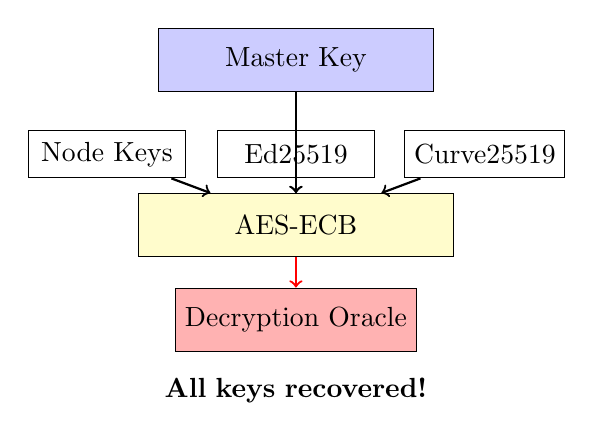
\begin{tikzpicture}[scale=0.6]
				\node[draw, rectangle, minimum width=3.5cm, minimum height=0.8cm, fill=blue!20] (master) at (0,4) {Master Key};

				% Encrypted items
				\node[draw, rectangle, minimum width=2cm, minimum height=0.6cm] (nodekeys) at (-4,2) {Node Keys};
				\node[draw, rectangle, minimum width=2cm, minimum height=0.6cm] (ed25519) at (0,2) {Ed25519};
				\node[draw, rectangle, minimum width=2cm, minimum height=0.6cm] (curve25519) at (4,2) {Curve25519};

				% AES-ECB
				\node[draw, rectangle, minimum width=4cm, minimum height=0.8cm, fill=yellow!20] (aesecb) at (0,0.5) {AES-ECB};

				\draw[->, thick] (master) -- (aesecb);
				\draw[->, thick] (nodekeys) -- (aesecb);
				\draw[->, thick] (ed25519) -- (aesecb);
				\draw[->, thick] (curve25519) -- (aesecb);

				% Attack
				\node[draw, rectangle, minimum width=3cm, minimum height=0.8cm, fill=red!30] (attack) at (0,-1.5) {Decryption Oracle};
				\draw[->, thick, red] (aesecb) -- (attack);

				% Result
				\node[text width=4cm, align=center] at (0,-3) {\textbf{All keys recovered!}};
			\end{tikzpicture}
		\end{column}
	\end{columns}
\end{frame}
\begin{frame}{MEGA attacks: Summary}
	\begin{center}
		\textbf{Note: Due to time constraints, we won't dive into the details of each attack}
	\end{center}
	\begin{columns}[c]
		\begin{column}{0.5\textwidth}
			\begin{itemize}
				\item \textbf{Attack 1 (RSA Key Recovery):} Exploit missing integrity protection to recover RSA private key in 512 logins\footnote{Later improved to 2 logins: \url{https://appliedcryptography.page/papers/\#mega-recovery}}
				\item \textbf{Attack 2 (Plaintext Recovery):} Use recovered RSA key to build AES-ECB decryption oracle for all encrypted keys
			\end{itemize}
		\end{column}
		\begin{column}{0.5\textwidth}
			\begin{itemize}
				\item \textbf{Attack 3a (File Integrity - Oracle):} Forge files using decryption oracle to frame users with malicious content
				\item \textbf{Attack 3b (File Integrity - Key Reuse):} Forge files without oracle by exploiting MEGA's key obfuscation scheme
				\item \textbf{Attack 4 (RSA Decryption):} Bleichenbacher's attack on PKCS\#1 v1.5 to decrypt RSA-encrypted keys
			\end{itemize}
		\end{column}
	\end{columns}
\end{frame}

\begin{frame}{MEGA attacks: Summary}
	\begin{columns}[c]
		\begin{column}{1\textwidth}
			\begin{table}
				\centering
				\small
				\begin{tabular}{|l|c|c|l|}
					\hline
					\textbf{Attack}    & \textbf{Attempts} & \textbf{Prerequisites} & \textbf{Impact}        \\
					\hline
					RSA Key Recovery   & 2 logins          & None                   & Share keys compromised \\
					\hline
					Plaintext Recovery & Varies            & Attack 1               & All keys compromised   \\
					\hline
					Integrity Attack A & 1                 & Attack 2               & File forgery           \\
					\hline
					Integrity Attack B & 1                 & One AES block          & File forgery           \\
					\hline
					RSA Decryption     & $2^{17}$          & Weaker model           & Chat/node keys         \\
					\hline
				\end{tabular}
			\end{table}
			\vspace{0.5cm}
			\textbf{Root causes:}
			\begin{itemize}
				\item No authenticated encryption (AES-ECB without MAC)
				\item Key reuse across different contexts
				\item Legacy cryptography (PKCS\#1 v1.5)
				\item \textbf{Complex, ad-hoc design without formal analysis!}
			\end{itemize}
		\end{column}
	\end{columns}
\end{frame}

\subsection{Attacks on Nextcloud}

\begin{frame}{Nextcloud: Overview}
	\begin{columns}[c]
		\begin{column}{0.75\textwidth}
			\begin{itemize}
				\item Open-source self-hosted cloud storage platform
				\item Founded in 2016 (fork of ownCloud)
				\item \textbf{Key statistics:}
				      \begin{itemize}
					      \item 20+ million users (2017)
					      \item 400,000+ deployments (2022)
					      \item Used by German government, Amnesty International
				      \end{itemize}
				\item \textbf{E2EE claims:}
				      \begin{itemize}
					      \item ``Zero Knowledge'' server
					      \item Secure against full server breach
					      \item Enterprise-grade encryption
				      \end{itemize}
			\end{itemize}
		\end{column}
		\begin{column}{0.25\textwidth}
			\imagewithcaption{nextcloud_logo.png}{Nextcloud's logo.}
		\end{column}
	\end{columns}
\end{frame}

\begin{frame}{Nextcloud: E2EE Design}
	\begin{columns}[c]
		\begin{column}{0.6\textwidth}
			\begin{itemize}
				\item E2EE is \textbf{not enabled by default}
				\item Users must manually mark folders as E2EE
				\item \textbf{Encryption approach:}
				      \begin{itemize}
					      \item Each file: AES-GCM with unique key
					      \item File keys encrypted by metadata key
					      \item Metadata keys encrypted by RSA-OAEP
				      \end{itemize}
				\item \textbf{Key rotation support:}
				      \begin{itemize}
					      \item Array of metadata keys per folder
					      \item Uses highest-indexed key for encryption
					      \item Re-encrypts on each sync
				      \end{itemize}
			\end{itemize}
		\end{column}
		\begin{column}{0.4\textwidth}
			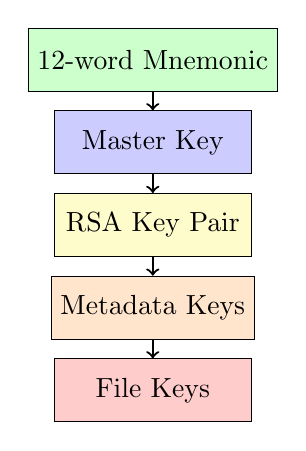
\begin{tikzpicture}[scale=0.7]
				% Mnemonic
				\node[draw, rectangle, minimum width=3cm, minimum height=0.8cm, fill=green!20] (mnemonic) at (0,5) {12-word Mnemonic};

				% Master key
				\node[draw, rectangle, minimum width=2.5cm, minimum height=0.8cm, fill=blue!20] (master) at (0,3.5) {Master Key};
				\draw[->, thick] (mnemonic) -- (master);

				% RSA keys
				\node[draw, rectangle, minimum width=2.5cm, minimum height=0.8cm, fill=yellow!20] (rsa) at (0,2) {RSA Key Pair};
				\draw[->, thick] (master) -- (rsa);

				% Metadata keys
				\node[draw, rectangle, minimum width=2.5cm, minimum height=0.8cm, fill=orange!20] (metadata) at (0,0.5) {Metadata Keys};
				\draw[->, thick] (rsa) -- (metadata);

				% File keys
				\node[draw, rectangle, minimum width=2.5cm, minimum height=0.8cm, fill=red!20] (filekeys) at (0,-1) {File Keys};
				\draw[->, thick] (metadata) -- (filekeys);
			\end{tikzpicture}
		\end{column}
	\end{columns}
\end{frame}

\begin{frame}{Nextcloud: Key hierarchy}
	\begin{columns}[c]
		\begin{column}{0.5\textwidth}
			\begin{itemize}
				\item \textbf{Mnemonic (top level):}
				      \begin{itemize}
					      \item 12 random words
					      \item Generated by client
					      \item User must memorize/store
				      \end{itemize}
				\item \textbf{Master key:}
				      \begin{itemize}
					      \item Derived from mnemonic
					      \item Encrypts RSA private key
				      \end{itemize}
				\item \textbf{RSA key pair:}
				      \begin{itemize}
					      \item Public key stored in clear
					      \item Private key encrypted on server
					      \item Used for sharing folders
				      \end{itemize}
			\end{itemize}
		\end{column}
		\begin{column}{0.5\textwidth}
			\begin{itemize}
				\item \textbf{Metadata keys:}
				      \begin{itemize}
					      \item One per E2EE folder
					      \item Encrypted with RSA-OAEP
					      \item Encrypts file keys and metadata
				      \end{itemize}
				\item \textbf{File keys (bottom level):}
				      \begin{itemize}
					      \item Unique per file
					      \item Random 128-bit AES key
					      \item Encrypted by metadata key
				      \end{itemize}
			\end{itemize}
		\end{column}
	\end{columns}
\end{frame}

\begin{frame}{Nextcloud vulnerabilities: Overview}
	\begin{columns}[c]
		\begin{column}{1\textwidth}
			\textbf{Three critical vulnerabilities found:}\footnote{\url{https://appliedcryptography.page/papers/\#nextcloud-break}}
			\begin{enumerate}
				\item \textbf{Key Insertion Attack}
				      \begin{itemize}
					      \item Server can substitute metadata keys
					      \item Exploits lack of authentication in RSA-OAEP
				      \end{itemize}
				\item \textbf{Ghost Key Attack}
				      \begin{itemize}
					      \item Forces client to use all-zero encryption key
					      \item Exploits missing bounds checking
				      \end{itemize}
				\item \textbf{IV Reuse in AES-GCM}
				      \begin{itemize}
					      \item Same IV used when files are modified
					      \item Enables plaintext recovery and forgery
				      \end{itemize}
			\end{enumerate}
		\end{column}
	\end{columns}
\end{frame}

\begin{frame}{Attack 1: Key Insertion Attack}
	\begin{columns}[c]
		\begin{column}{0.7\textwidth}
			\begin{itemize}
				\item \textbf{Root cause:} RSA-OAEP provides confidentiality but \textbf{not authentication}
				\item \textbf{Attack scenario:}
				      \begin{enumerate}
					      \item Server creates chosen metadata key
					      \item Encrypts it with user's RSA public key
					      \item Places ciphertext in user's folder
					      \item Triggers key rotation
				      \end{enumerate}
				\item \textbf{Impact:}
				      \begin{itemize}
					      \item Server knows metadata key
					      \item Can decrypt all file keys
					      \item Can insert/modify files
				      \end{itemize}
			\end{itemize}
		\end{column}
		\begin{column}{0.3\textwidth}
			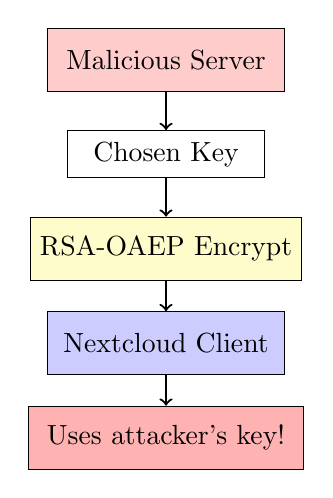
\begin{tikzpicture}[scale=0.8]
				% Malicious server
				\node[draw, rectangle, minimum width=3cm, minimum height=0.8cm, fill=red!20] (server) at (0,4) {Malicious Server};

				% Chosen key
				\node[draw, rectangle, minimum width=2.5cm, minimum height=0.6cm] (chosenkey) at (0,2.5) {Chosen Key};
				\draw[->, thick] (server) -- (chosenkey);

				% RSA-OAEP
				\node[draw, rectangle, minimum width=3cm, minimum height=0.8cm, fill=yellow!20] (rsaoaep) at (0,1) {RSA-OAEP Encrypt};
				\draw[->, thick] (chosenkey) -- (rsaoaep);

				% Client
				\node[draw, rectangle, minimum width=3cm, minimum height=0.8cm, fill=blue!20] (client) at (0,-0.5) {Nextcloud Client};
				\draw[->, thick] (rsaoaep) -- (client);

				% Result
				\node[draw, rectangle, minimum width=3.5cm, minimum height=0.8cm, fill=red!30] (result) at (0,-2) {Uses attacker's key!};
				\draw[->, thick] (client) -- (result);
			\end{tikzpicture}
		\end{column}
	\end{columns}
\end{frame}

\begin{frame}{The authentication problem in public key encryption}
	\begin{columns}[c]
		\begin{column}{1\textwidth}
			\begin{itemize}
				\item \textbf{What RSA-OAEP provides:}
				      \begin{itemize}
					      \item Confidentiality: Only private key holder can decrypt
					      \item Chosen-ciphertext security (IND-CCA2)
				      \end{itemize}
				\item \textbf{What RSA-OAEP does NOT provide:}
				      \begin{itemize}
					      \item Authentication: No proof of who created the ciphertext
					      \item Anyone with public key can encrypt
				      \end{itemize}
				\item \textbf{Nextcloud's assumption:}
				      \begin{itemize}
					      \item ``Only legitimate users will encrypt metadata keys''
					      \item But server has all public keys!
				      \end{itemize}
				\item \textbf{Solution approaches:}
				      \begin{itemize}
					      \item Digital signatures on encrypted keys
					      \item Authenticated encryption (e.g., signcryption)
					      \item Key exchange protocols instead of PKE
				      \end{itemize}
			\end{itemize}
		\end{column}
	\end{columns}
\end{frame}

\begin{frame}{Attack 2: Ghost Key Attack}
	\begin{columns}[c]
		\begin{column}{0.5\textwidth}
			\begin{itemize}
				\item \textbf{Vulnerability:} Missing bounds checking on metadata key array
				\item \textbf{Attack mechanism:}
				      \begin{enumerate}
					      \item Server modifies key index
					      \item Points to non-existent entry
					      \item Client allocates default key
					      \item Default is all zeros!
				      \end{enumerate}
				\item \textbf{Result:}
				      \begin{itemize}
					      \item Files encrypted with known key (0x00...)
					      \item Complete confidentiality loss
					      \item Trivial file forgery
				      \end{itemize}
			\end{itemize}
		\end{column}
		\begin{column}{0.5\textwidth}
			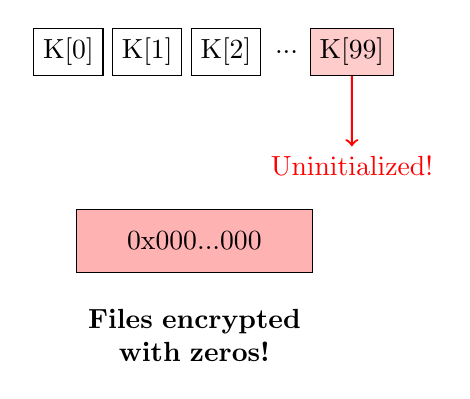
\begin{tikzpicture}[scale=0.8]
				% Key array
				\node[draw, rectangle, minimum width=0.8cm, minimum height=0.6cm] (key0) at (0,3) {K[0]};
				\node[draw, rectangle, minimum width=0.8cm, minimum height=0.6cm] (key1) at (1.25,3) {K[1]};
				\node[draw, rectangle, minimum width=0.8cm, minimum height=0.6cm] (key2) at (2.5,3) {K[2]};
				\node[right] at (3.125,3) {...};

				% Invalid index
				\node[draw, rectangle, minimum width=0.8cm, minimum height=0.6cm, fill=red!20] (keyX) at (4.5,3) {K[99]};

				% Arrow to ghost
				\draw[->, thick, red] (keyX) -- (4.5,1.5) node[below] {Uninitialized!};

				% All zeros
				\node[draw, rectangle, minimum width=3cm, minimum height=0.8cm, fill=red!30] (zeros) at (2,0) {0x000...000};

				% Result
				\node[text width=4cm, align=center] at (2,-1.5) {\textbf{Files encrypted with zeros!}};
			\end{tikzpicture}
		\end{column}
	\end{columns}
\end{frame}

\begin{frame}{Attack 3: IV Reuse in AES-GCM}
	\begin{columns}[c]
		\begin{column}{0.6\textwidth}
			\begin{itemize}
				\item \textbf{Critical flaw:} Same IV used when file is modified
				\item \textbf{AES-GCM requirement:} Never reuse IV with same key
				\item \textbf{Consequences of IV reuse:}
				      \begin{itemize}
					      \item Keystream repeats
					      \item XOR of plaintexts revealed
					      \item Authentication key recovery
				      \end{itemize}
				\item \textbf{Attack scenarios:}
				      \begin{itemize}
					      \item \textbf{Plaintext recovery:} If attacker knows one version
					      \item \textbf{Forgery:} Create valid ciphertexts
				      \end{itemize}
			\end{itemize}
		\end{column}
		\begin{column}{0.4\textwidth}
			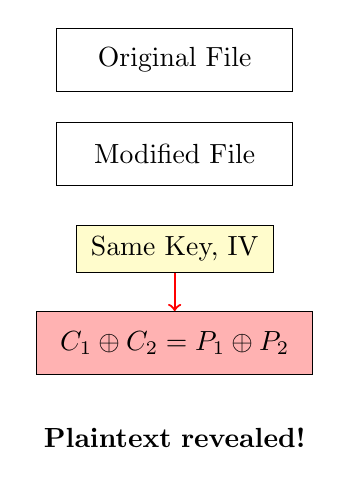
\begin{tikzpicture}[scale=0.8]
				% Original file
				\node[draw, rectangle, minimum width=3cm, minimum height=0.8cm] (file1) at (0,3) {Original File};

				% Modified file
				\node[draw, rectangle, minimum width=3cm, minimum height=0.8cm] (file2) at (0,1.5) {Modified File};

				% Same key and IV
				\node[draw, rectangle, minimum width=2.5cm, minimum height=0.6cm, fill=yellow!20] (keyiv) at (0,0) {Same Key, IV};

				% XOR reveals difference
				\node[draw, rectangle, minimum width=3.5cm, minimum height=0.8cm, fill=red!30] (xor) at (0,-1.5) {$C_1 \oplus C_2 = P_1 \oplus P_2$};
				\draw[->, thick, red] (keyiv) -- (xor);

				% Result
				\node[text width=3.5cm, align=center] at (0,-3) {\textbf{Plaintext revealed!}};
			\end{tikzpicture}
		\end{column}
	\end{columns}
\end{frame}

\begin{frame}{Nextcloud's response}
	\begin{columns}[c]
		\begin{column}{1\textwidth}
			\begin{itemize}
				\item \textbf{Initial patches:}
				      \begin{itemize}
					      \item Added bounds checking (Ghost Key)
					      \item Generate new IV on file modification
					      \item But Key Insertion attack remained...
				      \end{itemize}
				\item \textbf{Drastic measure (2023):}
				      \begin{itemize}
					      \item \textbf{Disabled E2EE file sharing entirely}
					      \item Could not fix authentication issues
					      \item Major feature regression
				      \end{itemize}
				\item \textbf{Lessons learned:}
				      \begin{itemize}
					      \item Ad-hoc crypto designs are dangerous
					      \item Retrofitting security is difficult
					      \item Need formal analysis before deployment
					      \item Authentication is as important as confidentiality
				      \end{itemize}
			\end{itemize}
		\end{column}
	\end{columns}
\end{frame}

\begin{frame}{Comparing MEGA and Nextcloud failures}
	\begin{columns}
		\begin{column}{0.5\textwidth}
			\textbf{MEGA}
			\vspace{0.3cm}
			\begin{itemize}
				\item No authenticated encryption
				\item Complex key hierarchy
				\item ECB mode usage
				\item Legacy crypto (PKCS\#1 v1.5)
				\item Patches partially successful
			\end{itemize}
		\end{column}
		\begin{column}{0.5\textwidth}
			\textbf{Nextcloud}
			\vspace{0.3cm}
			\begin{itemize}
				\item Missing authentication
				\item Implementation bugs
				\item IV reuse in AES-GCM
				\item Bounds checking errors
				\item Had to disable features
			\end{itemize}
		\end{column}
	\end{columns}
	\vspace{0.5cm}
	\begin{center}
		\textbf{Common theme:} Complex, ad-hoc designs without formal security analysis!
	\end{center}
\end{frame}

\section{Authentication: Moving Beyond Passwords}

\begin{frame}{Beyond password hashing: Zero-knowledge protocols}
	\begin{itemize}
		\item Password hashing has fundamental limitations:
		      \begin{itemize}
			      \item Server must receive password (or hash) to verify
			      \item Vulnerable to offline dictionary attacks
			      \item Trade-off between security and performance
		      \end{itemize}
		\item \textbf{Zero-knowledge password protocols} offer better security:
		      \begin{itemize}
			      \item Server never sees password or password-equivalent
			      \item No offline dictionary attacks possible
			      \item Cryptographic proof of password knowledge
		      \end{itemize}
	\end{itemize}
\end{frame}

\begin{frame}{SRP (Secure Remote Password)}
	\begin{itemize}
		\item Developed by Tom Wu at Stanford (1998)
		\item \textbf{Key properties:}
		      \begin{itemize}
			      \item Password never transmitted, even encrypted
			      \item Mutual authentication between client and server
			      \item Generates session key for subsequent encryption
			      \item Patent-free and standardized (RFC 2945)
		      \end{itemize}
		\item \textbf{How it works:}
		      \begin{itemize}
			      \item Registration: Client sends verifier derived from password
			      \item Authentication: Zero-knowledge proof using verifier
			      \item Based on discrete logarithm problem
		      \end{itemize}
		\item \textbf{Adoption:} Used by Apple iCloud, 1Password, ProtonMail
	\end{itemize}
\end{frame}

\begin{frame}{OPAQUE: Next-generation password authentication}
	\begin{itemize}
		\item Developed by Jarecki, Krawczyk, and Xu (2018)
		\item \textbf{Advantages over SRP:}
		      \begin{itemize}
			      \item Stronger security proofs in UC framework
			      \item Protection against pre-computation attacks
			      \item Forward secrecy for passwords
			      \item Quantum-resistant variants possible
		      \end{itemize}
		\item \textbf{Key innovation:} Oblivious PRF (OPRF)
		      \begin{itemize}
			      \item Server helps compute PRF without learning input
			      \item Prevents server from testing password guesses
		      \end{itemize}
		\item Being standardized by IETF (RFC 9497)
		\item Early adoption by WhatsApp for backup encryption
	\end{itemize}
\end{frame}

\begin{frame}{Signal's SVR3: Multi-enclave key recovery}
	\begin{columns}[c]
		\begin{column}{1\textwidth}
			\begin{itemize}
				\item Signal faced same challenge: E2EE backups need secure key recovery
				\item \textbf{SVR3 (Secure Value Recovery 3)\footnote{\url{https://appliedcryptography.page/papers/\#signal-recovery}}:} PIN-based key recovery
				      \begin{itemize}
					      \item Distributes trust across 3 different hardware enclaves
					      \item Intel SGX (Azure), AMD SEV-SNP (Google Cloud), Nitro (AWS)
					      \item Attacker must compromise ALL three to access keys
				      \end{itemize}
				\item \textbf{Key features:}
				      \begin{itemize}
					      \item Uses Password Protected Secret Sharing (PPSS)
					      \item Limits PIN guesses via secure hardware
					      \item No single point of failure
					      \item Cost: \$0.0025/user/year
				      \end{itemize}
				\item Already deployed to millions of Signal users
			\end{itemize}
		\end{column}
	\end{columns}
\end{frame}

\begin{frame}{Comparing authentication approaches}
	\begin{columns}
		\begin{column}{0.33\textwidth}
			\textbf{Password Hashing}
			\vspace{0.3cm}
			\begin{itemize}
				\item[\textcolor{green}{\mycheckmark}] Simple to implement
				\item[\textcolor{green}{\mycheckmark}] Well understood
				\item[\textcolor{red}{$\times$}] Offline attacks
				\item[\textcolor{red}{$\times$}] Server sees password
			\end{itemize}
		\end{column}
		\begin{column}{0.33\textwidth}
			\textbf{SRP}
			\vspace{0.3cm}
			\begin{itemize}
				\item[\textcolor{green}{\mycheckmark}] No offline attacks
				\item[\textcolor{green}{\mycheckmark}] Proven secure
				\item[\textcolor{orange}{$\sim$}] Complex protocol
				\item[\textcolor{red}{$\times$}] Pre-computation attacks
			\end{itemize}
		\end{column}
		\begin{column}{0.34\textwidth}
			\textbf{OPAQUE}
			\vspace{0.3cm}
			\begin{itemize}
				\item[\textcolor{green}{\mycheckmark}] Strongest security
				\item[\textcolor{green}{\mycheckmark}] Forward secrecy
				\item[\textcolor{red}{$\times$}] New protocol
				\item[\textcolor{red}{$\times$}] Limited deployment
			\end{itemize}
		\end{column}
	\end{columns}
	\vspace{0.5cm}
	\begin{center}
		\textit{For E2EE storage: Can derive encryption keys from authentication protocol outputs}
	\end{center}
\end{frame}

\begin{frame}{OPAQUE: How it works under the hood}
	\begin{columns}[c]
		\begin{column}{1\textwidth}
			\begin{itemize}
				\item \textbf{OPAQUE combines three key components:}
				      \begin{itemize}
					      \item \textbf{OPRF (Oblivious PRF):} Server helps compute function without seeing input
					      \item \textbf{Authenticated Key Exchange:} Derives session keys after password verification
					      \item \textbf{Password hardening:} Makes brute-force attacks computationally expensive
				      \end{itemize}
				\item \textbf{The magic:} Server stores a ``password file'' but:
				      \begin{itemize}
					      \item File doesn't contain password or hash
					      \item Server can't test password guesses offline
					      \item Client proves password knowledge without revealing it
					            \begin{itemize}
						            \item You could even say they perform a \textit{zero knowledge proof}!
					            \end{itemize}
				      \end{itemize}
			\end{itemize}
		\end{column}
	\end{columns}
\end{frame}

\begin{frame}{What is an OPRF?}{Oblivious Pseudorandom Function}
	\begin{columns}[c]
		\begin{column}{1\textwidth}
			\begin{itemize}
				\item \textbf{Definition:} A two-party protocol where:
				      \begin{itemize}
					      \item Client has input $x$
					      \item Server has key $k$
					      \item Client learns $F(k, x)$ and nothing else
					      \item Server learns nothing about $x$
					            \begin{itemize}
						            \item You could even say they perform a \textit{multi-party computation}!
					            \end{itemize}
				      \end{itemize}
				\item \textbf{Key properties:}
				      \begin{itemize}
					      \item \textbf{Oblivious:} Server doesn't learn client's input
					      \item \textbf{Verifiable:} Client can verify correct computation
					      \item \textbf{Deterministic:} Same input always gives same output
				      \end{itemize}
			\end{itemize}
		\end{column}
	\end{columns}
\end{frame}

\begin{frame}{OPAQUE Registration: Step by step}
	\begin{columns}[c]
		\begin{column}{0.5\textwidth}
			\textbf{Client actions:}
			\begin{enumerate}
				\item Choose password $pw$
				\item Run OPRF with server:\footnote{Here, our chosen OPRF operates in a cyclic group $\mathbb{G}$ of prime order $q$. The blinding factor $r$ is sampled uniformly at random from $\mathbb{Z}_q$, and $k$ is the server's OPRF key. I just made this OPRF up for the purposes of this slide and I don't know if it's secure (it probably is?)}
				      \begin{itemize}
					      \item Send blinded $H(pw)^r$
					      \item Get back $(H(pw)^r)^k$
					      \item Compute $rwd = H(pw)^k = (H(pw)^r)^{k/r}$
				      \end{itemize}
				\item Generate random private key $sk_c$
				\item Encrypt: $env = \text{Enc}(rwd, sk_c)$
				\item Send $(env, pk_c)$ to server
			\end{enumerate}
		\end{column}
		\begin{column}{0.5\textwidth}
			\textbf{Server actions:}
			\begin{enumerate}
				\item Generate OPRF key $k$
				\item Respond to OPRF:
				      \begin{itemize}
					      \item Receive blinded value
					      \item Return $(blinded)^k$
				      \end{itemize}
				\item Generate key pair $(sk_s, pk_s)$
				\item Store password file:
				      \begin{itemize}
					      \item Client's $env$ (encrypted)
					      \item Client's $pk_c$
					      \item Own $sk_s, pk_s$
					      \item OPRF key $k$
				      \end{itemize}
			\end{enumerate}
		\end{column}
	\end{columns}
\end{frame}

\begin{frame}{What's in the password file?}
	\begin{columns}[c]
		\begin{column}{0.6\textwidth}
			\begin{itemize}
				\item \textbf{Client's envelope ($env$):}
				      \begin{itemize}
					      \item Encrypted with $rwd = H(pw)^k$
					      \item Contains client's private key $sk_c$
					      \item Server can't decrypt without password
				      \end{itemize}
				\item \textbf{Public keys:}
				      \begin{itemize}
					      \item Client's $pk_c$ (for key exchange)
					      \item Server's $pk_s$ (for authentication)
				      \end{itemize}
				\item \textbf{Server's secrets:}
				      \begin{itemize}
					      \item OPRF key $k$ (for password evaluation)
					      \item Server private key $sk_s$
				      \end{itemize}
			\end{itemize}
		\end{column}
		\begin{column}{0.4\textwidth}
			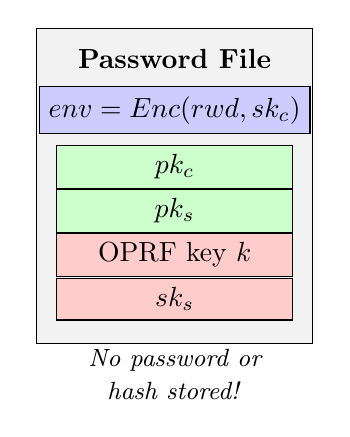
\begin{tikzpicture}[scale=0.8]
				% Password file box
				\node[draw, rectangle, minimum width=3.5cm, minimum height=4cm, fill=gray!10] (file) at (0,0) {};
				\node[above] at (0,1.7) {\textbf{Password File}};

				% Contents
				\node[draw, rectangle, minimum width=3cm, minimum height=0.6cm, fill=blue!20] (env) at (0,1.2) {$env = \text{Enc}(rwd, sk_c)$};
				\node[draw, rectangle, minimum width=3cm, minimum height=0.5cm, fill=green!20] (pkc) at (0,0.3) {$pk_c$};
				\node[draw, rectangle, minimum width=3cm, minimum height=0.5cm, fill=green!20] (pks) at (0,-0.4) {$pk_s$};
				\node[draw, rectangle, minimum width=3cm, minimum height=0.5cm, fill=red!20] (k) at (0,-1.1) {OPRF key $k$};
				\node[draw, rectangle, minimum width=3cm, minimum height=0.5cm, fill=red!20] (sks) at (0,-1.8) {$sk_s$};

				% Note
				\node[text width=3.5cm, align=center] at (0,-3) {\small\textit{No password or hash stored!}};
			\end{tikzpicture}
		\end{column}
	\end{columns}
\end{frame}

\begin{frame}{OPAQUE login (after registration)}
	\begin{columns}[c]
		\begin{column}{0.5\textwidth}
			\begin{itemize}
				\item[1.]\textbf{Client starts OPRF:}
				      \begin{itemize}
					      \item Blinds password: $\alpha = H(pw)^r$
					      \item Sends $\alpha$ to server
					      \item Note: This $r$ is freshly randomized - different from registration and each login
				      \end{itemize}
				\item[2.]\textbf{Server responds:}
				      \begin{itemize}
					      \item Computes $\beta = \alpha^k = H(pw)^{rk}$
					      \item Sends back $\beta$ and encrypted envelope $env$
				      \end{itemize}
			\end{itemize}
		\end{column}
		\begin{column}{0.5\textwidth}
			\begin{itemize}
				\item[3.]\textbf{Client recovers private key:}
				      \begin{itemize}
					      \item Unblinds: $rwd = \beta^{1/r} = H(pw)^k$
					      \item Decrypts: $sk_c = \text{Dec}(rwd, env)$
					      \item If wrong password, decryption fails!
				      \end{itemize}
				\item[4.]\textbf{Authenticated key exchange:}
				      \begin{itemize}
					      \item Client and server run AKE using their key pairs
					      \item Derives session key and export key
					      \item Mutual authentication achieved
				      \end{itemize}
			\end{itemize}
		\end{column}
	\end{columns}
\end{frame}

\begin{frame}{Why can't the server test passwords?}
	\begin{columns}[c]
		\begin{column}{0.5\textwidth}
			\textbf{What the server sees:}
			\begin{itemize}
				\item Random group element $\alpha$
				\item No relation to password visible
				\item Different $\alpha$ each login (random $r$)
				\item Can't extract $H(pw)$ from $\alpha$
			\end{itemize}
		\end{column}
		\begin{column}{0.5\textwidth}
			\textbf{What prevents offline attacks:}
			\begin{itemize}
				\item Server doesn't know $H(pw)$
				\item Can't verify guesses without client
				\item Each guess requires online interaction
				\item Rate limiting becomes enforceable
			\end{itemize}
		\end{column}
	\end{columns}
	\vspace{0.5cm}
	\begin{center}
		\textbf{Key insight:} The OPRF makes the server ``blind'' to the password while still enabling authentication
	\end{center}
\end{frame}

\begin{frame}{OPAQUE's security guarantees}
	\begin{columns}[c]
		\begin{column}{0.5\textwidth}
			\textbf{Against server compromise:}
			\begin{itemize}
				\item[\textcolor{green}{\mycheckmark}] No offline dictionary attacks
				\item[\textcolor{green}{\mycheckmark}] Forward secrecy for passwords
				\item[\textcolor{green}{\mycheckmark}] Past sessions remain secure
			\end{itemize}
		\end{column}
		\begin{column}{0.5\textwidth}
			\textbf{Against active attacks:}
			\begin{itemize}
				\item[\textcolor{green}{\mycheckmark}] Mutual authentication
				\item[\textcolor{green}{\mycheckmark}] Key confirmation
				\item[\textcolor{green}{\mycheckmark}] Protection from phishing
			\end{itemize}
		\end{column}
	\end{columns}
	\vspace{0.5cm}
	\begin{center}
		\textbf{Bonus:} Provides both authentication \textit{and} key derivation - perfect for E2EE storage!
	\end{center}
\end{frame}

\section{Case Study: WhatsApp End-to-End Encrypted Backups}

\subsection{WhatsApp's Design}

\begin{frame}{WhatsApp End-to-End Encrypted Backups: Overview}
	\begin{columns}[c]
		\begin{column}{0.75\textwidth}
			\begin{itemize}
				\item WhatsApp messages have been E2EE since 2016
				\item \textbf{Problem:} Backups in iCloud/Google Drive were not E2EE
				\item \textbf{Solution (2021):} End-to-end encrypted backups
				\item \textbf{Key innovation:} HSM-based Backup Key Vault
				      \begin{itemize}
					      \item Hardware Security Module for key storage
					      \item Password-protected key recovery
					      \item Brute-force protection
				      \end{itemize}
				\item \textbf{User choice:}
				      \begin{itemize}
					      \item Password-based recovery (via HSM)
					      \item 64-digit key (user manages)
				      \end{itemize}
			\end{itemize}
		\end{column}
		\begin{column}{0.25\textwidth}
			\imagewithcaption{whatsapp_logo.png}{WhatsApp logo.}
		\end{column}
	\end{columns}
\end{frame}

\begin{frame}{The backup encryption challenge}
	\begin{columns}[c]
		\begin{column}{1\textwidth}
			\begin{itemize}
				\item \textbf{User expectations:}
				      \begin{itemize}
					      \item Recover chats after losing phone
					      \item Transfer chats to new device
					      \item No complex key management
				      \end{itemize}
				\item \textbf{Security requirements:}
				      \begin{itemize}
					      \item WhatsApp cannot read backups
					      \item Cloud providers cannot read backups
					      \item Protection against brute-force attacks
				      \end{itemize}
				\item \textbf{Traditional approach:} Trust cloud provider
				\item \textbf{WhatsApp's approach:} Client-side encryption with secure key recovery
			\end{itemize}
		\end{column}
	\end{columns}
\end{frame}

\begin{frame}{Hardware Security Modules (HSMs)}{What are they?}
	\begin{columns}[c]
		\begin{column}{0.4\textwidth}
			\begin{itemize}
				\item \textbf{Definition:} Dedicated cryptographic processors designed for key protection
				\item \textbf{Key features:}
				      \begin{itemize}
					      \item Hardware-based key storage and generation
					      \item Tamper-resistant physical security
					      \item Cryptographic operations in secure boundary
					      \item FIPS 140-2 Level 3/4 certified
				      \end{itemize}
			\end{itemize}
		\end{column}
		\begin{column}{0.6\textwidth}
			\begin{itemize}
				\item \textbf{Security properties:}
				      \begin{itemize}
					      \item Keys never exist in plaintext outside HSM
					      \item Physical intrusion triggers key deletion
					      \item Rate limiting and access controls
					      \item Audit logging of all operations
				      \end{itemize}
				\item \textbf{Common uses:}
				      \begin{itemize}
					      \item PKI root certificate authorities
					      \item Payment card industry (PIN verification)
					      \item Database encryption key management
					      \item Code signing for software integrity
				      \end{itemize}
			\end{itemize}
		\end{column}
	\end{columns}
\end{frame}

\begin{frame}{HSM-based Backup Key Vault: The safe deposit box analogy}
	\begin{columns}[c]
		\begin{column}{0.5\textwidth}
			\textbf{Traditional Bank Safe Deposit Box}
			\begin{itemize}
				\item User has unique key
				\item Bank cannot open box
				\item Requires physical presence
				\item Lost key = lost contents
			\end{itemize}
		\end{column}
		\begin{column}{0.5\textwidth}
			\textbf{WhatsApp's Key Vault}
			\begin{itemize}
				\item Password protects key
				\item WhatsApp cannot access
				\item Remote recovery possible
				\item Password attempts limited
			\end{itemize}
		\end{column}
	\end{columns}
\end{frame}

\begin{frame}{System architecture}
	\begin{columns}[c]
		\begin{column}{0.6\textwidth}
			\begin{itemize}
				\item \textbf{Client side:}
				      \begin{itemize}
					      \item $K \twoheadleftarrow \bits^{256}$
					      \item Encrypts backup with $K$
					      \item Uploads to iCloud/Google Drive
				      \end{itemize}
				\item \textbf{WhatsApp infrastructure:}
				      \begin{itemize}
					      \item Front-end service (ChatD)
					      \item HSM-based Backup Key Vault
					      \item Geographically distributed
				      \end{itemize}
				\item \textbf{Security properties:}
				      \begin{itemize}
					      \item Cloud provider sees only ciphertext
					      \item $K$ never leaves client unencrypted
					      \item Password never known to WhatsApp
				      \end{itemize}
			\end{itemize}
		\end{column}
		\begin{column}{0.4\textwidth}
			\imagewithcaption{whatsapp_backups.png}{Source: \url{https://appliedcryptography.page/papers/\#whatsapp-backups}}
		\end{column}
	\end{columns}
\end{frame}

\begin{frame}{Now the problem becomes: how to store encrypted $K$?}
	\begin{columns}[c]
		\begin{column}{0.5\textwidth}
			\begin{itemize}
				\item WhatsApp uses OPAQUE for password-based key storage
				\item \textbf{Key properties of OPAQUE:}
				      \begin{itemize}
					      \item Server never learns password
					      \item No offline dictionary attacks
					      \item Derives encryption key from password
					      \item Strong security proofs
				      \end{itemize}
			\end{itemize}
		\end{column}
		\begin{column}{0.5\textwidth}
			\begin{itemize}
				\item \textbf{How it works:}
				      \begin{itemize}
					      \item Registration: Client creates password-protected record
					      \item Retrieval: Client proves password knowledge
					      \item Server helps compute key without learning password
				      \end{itemize}
				\item \textbf{Advantage over simple password hashing:}
				      \begin{itemize}
					      \item HSM enforces rate limiting
					      \item No password-equivalent stored
				      \end{itemize}
			\end{itemize}
		\end{column}
	\end{columns}
\end{frame}

\begin{frame}{Registration process}
	\begin{columns}[c]
		\begin{column}{1\textwidth}
			\begin{enumerate}
				\item User enters password
				\item Client starts OPAQUE registration
				\item Server returns registration response + signature
				\item Client completes registration:
				      \begin{itemize}
					      \item Derives $\mathtt{OPAQUE}_K$
					      \item Sends $\func{aes-gcm}{\mathtt{OPAQUE}_K, K}$ to server
				      \end{itemize}
				\item Server stores encrypted record
			\end{enumerate}
		\end{column}
	\end{columns}
\end{frame}

\begin{frame}{Key retrieval process}
	\begin{columns}[c]
		\begin{column}{0.6\textwidth}
			\begin{enumerate}
				\item Client initiates OPAQUE login with password
				\item Server decrements attempt counter
				\item Server returns credential response
				\item Client completes login:
				      \begin{itemize}
					      \item Derives $\mathtt{SHARED}_K$ and $\mathtt{OPAQUE}_K$
					      \item Sends finalization message
				      \end{itemize}
				\item Server returns encrypted key ($EK$)
				\item Client decrypts:
				      \begin{itemize}
					      \item First with $\mathtt{SHARED}_K$
					      \item Then with $\mathtt{OPAQUE}_K$
					      \item Recovers backup key K
				      \end{itemize}
			\end{enumerate}
		\end{column}
		\begin{column}{0.4\textwidth}
			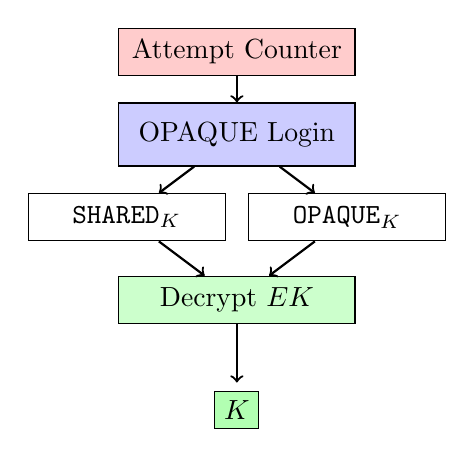
\begin{tikzpicture}[scale=0.7]
				% Attempt counter
				\node[draw, rectangle, minimum width=3cm, minimum height=0.6cm, fill=red!20] (counter) at (0,4) {Attempt Counter};

				% OPAQUE login
				\node[draw, rectangle, minimum width=3cm, minimum height=0.8cm, fill=blue!20] (opaque) at (0,2.5) {OPAQUE Login};
				\draw[->, thick] (counter) -- (opaque);

				% Keys derived
				\node[draw, rectangle, minimum width=2.5cm, minimum height=0.6cm] (shared) at (-2,1) {$\mathtt{SHARED}_K$};
				\node[draw, rectangle, minimum width=2.5cm, minimum height=0.6cm] (opaquek) at (2,1) {$\mathtt{OPAQUE}_K$};
				\draw[->, thick] (opaque) -- (shared);
				\draw[->, thick] (opaque) -- (opaquek);

				% Decryption
				\node[draw, rectangle, minimum width=3cm, minimum height=0.6cm, fill=green!20] (decrypt) at (0,-0.5) {Decrypt $EK$};
				\draw[->, thick] (shared) -- (decrypt);
				\draw[->, thick] (opaquek) -- (decrypt);

				% Result
				\node[draw, rectangle, fill=green!30] at (0,-2.5) {$K$};
				\draw[->, thick] (decrypt) -- (0,-2);
			\end{tikzpicture}
		\end{column}
	\end{columns}
\end{frame}

\begin{frame}{Security features}
	\begin{columns}[c]
		\begin{column}{0.5\textwidth}
			\textbf{Brute-force protection}
			\begin{itemize}
				\item HSM enforces attempt limits
				\item After threshold: Key permanently inaccessible
				\item Rate limiting in hardware
			\end{itemize}
		\end{column}
		\begin{column}{0.5\textwidth}
			\textbf{Infrastructure resilience}
			\begin{itemize}
				\item 5 datacenter deployment
				\item Majority consensus system
				\item Tolerates multiple failures
				\item Geographic distribution
			\end{itemize}
		\end{column}
	\end{columns}
	\vspace{0.5cm}
	\begin{center}
		\textbf{Transport security:} Noise Protocol Framework for client-server communication (here used as an alternative to TLS, but in reality it's a whole thing that lets you design a versatile amount of protocols)
	\end{center}
\end{frame}

\begin{frame}{Alternative: User-managed 64-digit key}
	\begin{columns}[c]
		\begin{column}{1\textwidth}
			\begin{itemize}
				\item \textbf{For users who prefer full control:}
				      \begin{itemize}
					      \item 64-digit encryption key option
					      \item Key never sent to WhatsApp
					      \item User must store key securely
				      \end{itemize}
				\item \textbf{Trade-offs:}
				      \begin{itemize}
					      \item[\textcolor{green}{\mycheckmark}] Maximum security - no trust required
					      \item[\textcolor{green}{\mycheckmark}] No brute-force risk
					      \item[\textcolor{red}{$\times$}] User responsibility for key management
					      \item[\textcolor{red}{$\times$}] Lost key = lost backups forever
				      \end{itemize}
				\item \textbf{Recommendation:} Only for technically sophisticated users
			\end{itemize}
		\end{column}
	\end{columns}
\end{frame}

\begin{frame}{WhatsApp's design principles}
	\begin{columns}[c]
		\begin{column}{1\textwidth}
			\begin{itemize}
				\item \textbf{Use proven protocols:} OPAQUE for password authentication
				\item \textbf{Hardware security:} HSMs for tamper-resistant key storage
				\item \textbf{Defense in depth:}
				      \begin{itemize}
					      \item Client-side encryption
					      \item Zero-knowledge password protocol
					      \item Rate limiting in hardware
					      \item Geographic distribution
				      \end{itemize}
				\item \textbf{User choice:} Password vs self-managed key
				\item \textbf{Clear threat model:}
				      \begin{itemize}
					      \item Protects against cloud provider access
					      \item Protects against WhatsApp compromise
					      \item Limits brute-force attacks
				      \end{itemize}
			\end{itemize}
		\end{column}
	\end{columns}
\end{frame}

\begin{frame}{Lessons from WhatsApp's approach}
	\begin{columns}[c]
		\begin{column}{0.5\textwidth}
			\textbf{What they did right:}
			\begin{itemize}
				\item Used established OPAQUE protocol
				\item Hardware-backed security
				\item Simple, clear design
				\item Published detailed whitepaper
				\item Gradual rollout with testing
			\end{itemize}
		\end{column}
		\begin{column}{0.5\textwidth}
			\textbf{Key takeaways:}
			\begin{itemize}
				\item Don't reinvent authentication
				\item User education is crucial
				\item Transparency builds trust
				\item Complexity should be hidden
			\end{itemize}
		\end{column}
	\end{columns}
	\vspace{0.5cm}
	\begin{center}
		\textit{Compare with MEGA/Nextcloud: Standard protocols vs. custom designs}
	\end{center}
\end{frame}

\subsection{Critiquing WhatsApp's Design}

\begin{frame}{Specification ambiguity: A major flaw}
	\begin{columns}[c]
		\begin{column}{1\textwidth}
			\begin{itemize}
				\item \textbf{The problem:} WhatsApp's specification is ambiguous about $\mathtt{OPAQUE}_K$
				\item \textbf{Two possible interpretations:}
				      \begin{itemize}
					      \item \textbf{Option 1:} OPAQUE's export key (client-only secret)
					      \item \textbf{Option 2:} OPAQUE's shared session key (known to both parties)
				      \end{itemize}
				\item \textbf{Why this matters:}
				      \begin{itemize}
					      \item If Option 2: Server learns $\mathtt{OPAQUE}_K$
					      \item Server could decrypt backup key directly!
					      \item Completely breaks the security model
				      \end{itemize}
				\item \textbf{This type of ambiguity is dangerous:}
				      \begin{itemize}
					      \item Different implementations may choose differently
					      \item Security analysis becomes impossible
					      \item Opens door to implementation vulnerabilities
				      \end{itemize}
				\item \textbf{Lesson:} Cryptographic specifications must be \textit{unambiguous}
			\end{itemize}
		\end{column}
	\end{columns}
\end{frame}

\begin{frame}{Critical limitation: Trust in WhatsApp's infrastructure}
	\begin{columns}[c]
		\begin{column}{1\textwidth}
			\begin{itemize}
				\item \textbf{The fundamental trust problem:}
				      \begin{itemize}
					      \item WhatsApp claims to use HSMs, but users cannot verify
					      \item HSMs are owned and operated by WhatsApp
					      \item No independent audit or verification possible
					      \item Could be software emulation instead
				      \end{itemize}
				\item \textbf{What users must trust:}
				      \begin{itemize}
					      \item WhatsApp actually deployed HSMs as described
					      \item HSMs are configured correctly
					      \item Rate limiting is enforced as claimed
					      \item WhatsApp doesn't have backdoor access
				      \end{itemize}
			\end{itemize}
		\end{column}
	\end{columns}
\end{frame}

\begin{frame}{The HSM security theater problem}
	\begin{columns}[c]
		\begin{column}{0.5\textwidth}
			\textbf{What WhatsApp claims:}
			\begin{itemize}
				\item Hardware-enforced rate limiting
				\item Tamper-resistant key storage
				\item Geographic distribution
				\item No backdoor access
			\end{itemize}
		\end{column}
		\begin{column}{0.5\textwidth}
			\textbf{What users can verify:}
			\begin{itemize}
				\item Nothing!
				\item No attestation provided
				\item No third-party audits
				\item Closed-source implementation
			\end{itemize}
		\end{column}
	\end{columns}
\end{frame}

\begin{frame}{Potential vulnerabilities in WhatsApp's design}
	\begin{columns}[c]
		\begin{column}{1\textwidth}
			\begin{itemize}
				\item \textbf{Silent key escrow:}
				      \begin{itemize}
					      \item HSM could have backdoor for data extraction
					      \item HSM could literally be one guy in a basement memorizing everything
					      \item No way for users to detect this
				      \end{itemize}
				\item \textbf{Selective targeting:}
				      \begin{itemize}
					      \item Different behavior for specific accounts
					      \item Disable rate limiting for law enforcement
					      \item Return fake ``attempt exceeded'' to user
				      \end{itemize}
				\item \textbf{Implementation substitution:}
				      \begin{itemize}
					      \item Replace HSM with software for some users
					      \item Use weaker entropy for key generation
					      \item Log passwords before OPAQUE processing
				      \end{itemize}
			\end{itemize}
		\end{column}
	\end{columns}
\end{frame}

\begin{frame}{The attestation problem}
	\begin{columns}[c]
		\begin{column}{0.5\textwidth}
			\begin{itemize}
				\item \textbf{What's missing:}
				      \begin{itemize}
					      \item Remote attestation from HSMs
					      \item Cryptographic proof of HSM usage
					      \item Public audit logs
					      \item Third-party verification
				      \end{itemize}
				\item \textbf{Technical solutions exist:}
				      \begin{itemize}
					      \item HSMs can provide attestation
					      \item Intel SGX, AMD SEV offer remote attestation
					      \item Blockchain for public audit logs
				      \end{itemize}
			\end{itemize}
		\end{column}
		\begin{column}{0.5\textwidth}
			\begin{itemize}
				\item \textbf{Why not implemented?}
				      \begin{itemize}
					      \item Complexity for users?
					      \item Business reasons?
					      \item Legal requirements?
					      \item Law enforcement pressure?
				      \end{itemize}
			\end{itemize}
		\end{column}
	\end{columns}
\end{frame}

\begin{frame}{Law enforcement pressure?}
	\begin{columns}[c]
		\begin{column}{0.5\textwidth}
			\imagewithcaption{cloud_pressure_a.png}{Source: Reuters}
		\end{column}
		\begin{column}{0.5\textwidth}
			\imagewithcaption{cloud_pressure_b.png}{Source: \url{https://support.apple.com/en-us/122234}}
		\end{column}
	\end{columns}
\end{frame}

\begin{frame}{The 64-digit key mystery}
	\begin{columns}[c]
		\begin{column}{0.5\textwidth}
			\begin{itemize}
				\item \textbf{Why 64 digits?}
				      \begin{itemize}
					      \item 64 digits = ~212 bits of entropy
					      \item Much more than needed for 128-bit AES key
					      \item Difficult for humans to manage
					      \item Error-prone to transcribe
				      \end{itemize}
				\item \textbf{We already have better solutions:}
				      \begin{itemize}
					      \item BIP39 mnemonic phrases (12-24 words)\footnote{Argument against: hard to localize into many languages}
					      \item Used successfully by cryptocurrency wallets
					      \item Easier to write down and verify
					      \item Built-in error detection
				      \end{itemize}
			\end{itemize}
		\end{column}
		\begin{column}{0.5\textwidth}
			\begin{itemize}
				\item \textbf{Possible explanations:}
				      \begin{itemize}
					      \item Deliberate friction to push HSM option?
					      \item Making self-custody intentionally hard?
				      \end{itemize}
			\end{itemize}
		\end{column}
	\end{columns}
\end{frame}

\begin{frame}{A more honest assessment of WhatsApp backups}
	\begin{columns}[c]
		\begin{column}{1\textwidth}
			\begin{itemize}
				\item \textbf{What WhatsApp backups actually provide:}
				      \begin{itemize}
					      \item Protection from cloud providers (Google/Apple)
					      \item Some protection from external hackers
					      \item Convenient key recovery
				      \end{itemize}
				\item \textbf{What they DON'T provide:}
				      \begin{itemize}
					      \item Full protection from WhatsApp itself
					      \item Fully verifiable security guarantees
				      \end{itemize}
				\item \textbf{Alternatives:}
				      \begin{itemize}
					      \item Threshold cryptography across providers
					      \item Client-side key derivation only
					      \item Transparent, auditable systems
				      \end{itemize}
			\end{itemize}
		\end{column}
	\end{columns}
\end{frame}

\section{Designing an End-to-End Cloud Storage Protocol}

\subsection{Lessons Learned}

\begin{frame}{Lessons from MEGA and Nextcloud failures}
	\begin{columns}[c]
		\begin{column}{1\textwidth}
			\textbf{What went wrong?}
			\begin{itemize}
				\item \textbf{Ad-hoc design:} Both created custom cryptographic protocols
				\item \textbf{No formal analysis:} Security claims without proofs
				\item \textbf{Complexity spiral:} Features added without security review
				\item \textbf{Missing fundamentals:}
				      \begin{itemize}
					      \item MEGA: No authenticated encryption
					      \item Nextcloud: No sender authentication
					      \item Both: Improper use of cryptographic primitives
				      \end{itemize}
				\item \textbf{Patch difficulties:}
				      \begin{itemize}
					      \item MEGA: Multiple rounds of incomplete fixes
					      \item Nextcloud: Had to disable core features
				      \end{itemize}
			\end{itemize}
		\end{column}
	\end{columns}
\end{frame}

\begin{frame}{The danger of ad-hoc designs}
	\begin{columns}[c]
		\begin{column}{1\textwidth}
			\begin{itemize}
				\item \textbf{Common mistakes in ad-hoc designs:}
				      \begin{itemize}
					      \item Misunderstanding primitive guarantees
					      \item Ignoring composition problems
					      \item No clear threat model
					      \item Feature creep without security analysis
				      \end{itemize}
				\item \textbf{Why it happens:}
				      \begin{itemize}
					      \item Overconfidence in understanding
					      \item Time/resource constraints
					      \item Lack of cryptographic expertise
					      \item ``It encrypts, so it's secure''
				      \end{itemize}
			\end{itemize}
		\end{column}
	\end{columns}
\end{frame}

\begin{frame}{Principles of secure protocol design}
	\begin{columns}[c]
		\begin{column}{1\textwidth}
			\begin{enumerate}
				\item \textbf{Start with a clear threat model}
				      \begin{itemize}
					      \item What are you protecting against?
					      \item What can the adversary do?
					      \item What are acceptable trade-offs?
				      \end{itemize}
				\item \textbf{Use established cryptographic patterns}
				      \begin{itemize}
					      \item Authenticated encryption (AES-GCM, ChaCha20-Poly1305)
					      \item Standard key exchange (X3DH, Noise Protocol Framework)
					      \item Proven constructions (don't invent new ones!)
				      \end{itemize}
				\item \textbf{Keep it simple}
				      \begin{itemize}
					      \item Complexity is the enemy of security
					      \item Each feature multiplies attack surface
					      \item Can you explain your protocol in one page?
				      \end{itemize}
			\end{enumerate}
		\end{column}
	\end{columns}
\end{frame}

\begin{frame}{Reminder: formal analysis}
	\begin{columns}[c]
		\begin{column}{0.5\textwidth}
			\begin{itemize}
				\item \textbf{What is formal analysis?}\footnote{Coming soon in our upcoming topic sessions on High-Assurance Cryptography!}
				      \begin{itemize}
					      \item Automated using software
					      \item Mathematical proofs of security
					      \item Clear security definitions
					      \item Reduction to hard problems
					      \item Machine-verified proofs
				      \end{itemize}
				\item \textbf{Benefits:}
				      \begin{itemize}
					      \item Catches subtle flaws
					      \item Provides confidence
					      \item Clear security guarantees
					      \item Guides implementation
				      \end{itemize}
			\end{itemize}
		\end{column}
		\begin{column}{0.5\textwidth}
			\begin{itemize}
				\item \textbf{Types of analysis:}
				      \begin{itemize}
					      \item \textbf{Computational:} Reduction to hard problems
					      \item \textbf{Symbolic:} Protocol logic verification
					      \item \textbf{UC Framework:} Composable security
					      \item \textbf{Game-based:} Step-by-step proofs
				      \end{itemize}
				\item \textbf{Tools available:}
				      \begin{itemize}
					      \item ProVerif, Tamarin
					      \item EasyCrypt, CryptoVerif
					      \item \fstar
				      \end{itemize}
			\end{itemize}
		\end{column}
	\end{columns}
\end{frame}

\begin{frame}{Security definitions matter}
	\begin{columns}[c]
		\begin{column}{1\textwidth}
			\textbf{MEGA's mistake:} Assumed encryption provides integrity
			\begin{itemize}
				\item Used AES-ECB without MAC
				\item Encryption $\neq$ Authenticated encryption
				\item Led to complete key recovery
			\end{itemize}
			\textbf{Nextcloud's mistake:} Assumed encryption provides authentication
			\begin{itemize}
				\item RSA-OAEP only provides confidentiality
				\item Anyone can create valid ciphertexts
				\item Led to key insertion attacks
			\end{itemize}
			\textbf{Lesson:} Understand exactly what each primitive guarantees!
		\end{column}
	\end{columns}
\end{frame}

\begin{frame}{Protocol design methodology}
	\begin{columns}[c]
		\begin{column}{0.5\textwidth}
			\begin{itemize}
				\item \textbf{Requirements gathering}
				      \begin{itemize}
					      \item Security goals (confidentiality, integrity, authentication)
					      \item Functionality requirements
					      \item Performance constraints
				      \end{itemize}
				\item \textbf{Threat modeling}
				      \begin{itemize}
					      \item Define adversary capabilities
					      \item Identify trust assumptions
					      \item Document acceptable risks
				      \end{itemize}
			\end{itemize}
		\end{column}
		\begin{column}{0.5\textwidth}
			\begin{itemize}
				\item \textbf{Protocol design}
				      \begin{itemize}
					      \item Use standard building blocks
					      \item Create formal specification
					      \item Keep complexity minimal
				      \end{itemize}
				\item \textbf{Security analysis}
				      \begin{itemize}
					      \item Formal proofs or verification
					      \item External review
					      \item Test edge cases
				      \end{itemize}
			\end{itemize}
		\end{column}
	\end{columns}
\end{frame}

\begin{frame}{Learning from other successful protocols}
	\begin{columns}[c]
		\begin{column}{0.5\textwidth}
			\begin{itemize}
				\item \textbf{Signal Protocol}
				      \begin{itemize}
					      \item Formal security proofs
					      \item Clear threat model
					      \item Simple, modular design
					      \item Widely analyzed
				      \end{itemize}
				\item \textbf{WireGuard}
				      \begin{itemize}
					      \item Minimal codebase
					      \item Fixed crypto choices
					      \item Formal verification
					      \item Clear specification
				      \end{itemize}
			\end{itemize}
		\end{column}
		\begin{column}{0.5\textwidth}
			\begin{itemize}
				\item \textbf{TLS 1.3}
				      \begin{itemize}
					      \item Removed legacy features
					      \item Formal analysis during design
					      \item Simplified handshake
					      \item Clear security properties
				      \end{itemize}
				\item \textbf{Common themes:}
				      \begin{itemize}
					      \item Simplicity over features
					      \item Formal analysis early
					      \item Clear documentation
					      \item Conservative choices
				      \end{itemize}
			\end{itemize}
		\end{column}
	\end{columns}
\end{frame}

\begin{frame}{Key takeaways for protocol designers}
	\begin{columns}[c]
		\begin{column}{0.5\textwidth}
			\begin{itemize}
				\item \textbf{Don't roll your own crypto}
				      \begin{itemize}
					      \item Use established, analyzed protocols
					      \item If you must innovate, get expert review
				      \end{itemize}
				\item \textbf{Security is not just encryption}
				      \begin{itemize}
					      \item Authentication, integrity equally important
					      \item Consider key management, revocation
				      \end{itemize}
			\end{itemize}
		\end{column}
		\begin{column}{0.5\textwidth}
			\begin{itemize}
				\item \textbf{Formal analysis is worth it}
				      \begin{itemize}
					      \item Catches issues before deployment
					      \item Provides clear security guarantees
				      \end{itemize}
				\item \textbf{Simplicity is security}
				      \begin{itemize}
					      \item Every feature adds complexity
					      \item Complex protocols have more bugs
				      \end{itemize}
				\item \textbf{Learn from failures}
				      \begin{itemize}
					      \item Study what went wrong
					      \item Apply lessons to new designs
				      \end{itemize}
			\end{itemize}
		\end{column}
	\end{columns}
\end{frame}

\subsection{A Formal Treatment of End-to-End Encrypted Cloud Storage}

\begin{frame}{Next: A formal treatment from the literature}
	\begin{center}
		\textbf{What follows is based on:}\\
		\vspace{0.3cm}
		\textit{``A Formal Treatment of End-to-End Encrypted Cloud Storage''}\\
		{\tiny\url{https://appliedcryptography.page/papers/\#cloud-storage}}\\
		\vspace{0.2cm}
		{\small by Matilda Backendal, Hannah Davis, Felix Günther, Miro Haller, and Kenneth G. Paterson}
	\end{center}
	\begin{columns}[t]
		\begin{column}{0.5\textwidth}
			\begin{itemize}
				\item \textbf{Why this paper?}
				      \begin{itemize}
					      \item First comprehensive formal treatment of E2EE cloud storage
					      \item Addresses the exact failures we've seen in MEGA/Nextcloud
					      \item Shows how to do protocol design \textit{right}
				      \end{itemize}
			\end{itemize}
		\end{column}
		\begin{column}{0.5\textwidth}
			\begin{itemize}
				\item \textbf{Key contributions:}
				      \begin{itemize}
					      \item Formal security definitions for E2EE storage
					      \item Clean, analyzable protocol design
					      \item Security proofs in the UC framework
				      \end{itemize}
			\end{itemize}
		\end{column}
	\end{columns}
\end{frame}

\begin{frame}{A formal treatment: Building blocks}
	\begin{columns}[c]
		\begin{column}{1\textwidth}
			\textbf{Core cryptographic primitives:}
			\begin{itemize}
				\item \textbf{PRF (Pseudorandom Function):} $F: \{0,1\}^{kl} \times \{0,1\}^* \to \{0,1\}^{kl}$
				\item \textbf{MAC (Message Authentication Code):} For integrity verification
				\item \textbf{AEAD (Authenticated Encryption):} AES-GCM or ChaCha20-Poly1305
				\item \textbf{2HashDH OPRF:} Password hardening against offline attacks
			\end{itemize}
			\vspace{0.3cm}
			\textbf{Key insight:} Use standard, proven primitives - don't invent new ones!
		\end{column}
	\end{columns}
\end{frame}

\begin{frame}{The 2HashDH OPRF: Motivation}
	\begin{columns}[c]
		\begin{column}{1\textwidth}
			\begin{itemize}
				\item \textbf{Problem:} How to derive keys from passwords without server learning them?
				\item \textbf{Challenge:} Server needs to help with computation, but shouldn't learn password
				\item \textbf{Solution:} Oblivious Pseudorandom Function (OPRF) (Similar to OPAQUE)
				      \begin{itemize}
					      \item Client has secret input (account ID + password)
					      \item Server has key $k$
					      \item Together compute $F(k, \text{input})$ without server learning input
				      \end{itemize}
				\item \textbf{In our protocol:}
				      \begin{itemize}
					      \item Client generates OPRF key during registration
					      \item Sends key to server (ensures honest key generation)
					      \item Later uses OPRF to derive keys from password
				      \end{itemize}
			\end{itemize}
		\end{column}
	\end{columns}
\end{frame}

\begin{frame}{The 2HashDH OPRF: How it works}
	\begin{columns}[c]
		\begin{column}{1\textwidth}
			\textbf{Setup:} Group $\mathbb{G}$ of prime order $q$, hash functions $H_1$ and $H_2$\footnote{Ideally memory-hard and slow}
			\begin{itemize}
				\item \textbf{Goal:} Client computes $H_2(x, H_1(x)^k)$ without revealing $x$ to server
				\item \textbf{Protocol steps:}
				      \begin{enumerate}
					      \item Client picks random blinding factor $r \twoheadleftarrow \mathbb{Z}_q$
					      \item Client sends blinded value: $\alpha = H_1(x)^r$ to server
						            {\footnotesize\begin{itemize}
								            \item Client hashes their secret input $x$ to get $H_1(x)$, raises it to the power of $r$, and sends this ``blinded'' result to the server - the server cannot determine $x$ from this
							            \end{itemize}}
					      \item Server computes: $\beta = \alpha^k = H_1(x)^{rk}$ and returns it
					      \item Client unblinds: $\beta^{1/r} = H_1(x)^k$
					            {\footnotesize\begin{itemize}
								            \item The client removes the blinding by raising the server's response to the power of $1/r$ (the multiplicative inverse of $r$), which cancels out the $r$ in the exponent, leaving just $H_1(x)^k$
							            \end{itemize}}
					      \item Client outputs: $y = H_2(x, \beta^{1/r})$
				      \end{enumerate}
			\end{itemize}
		\end{column}
	\end{columns}
\end{frame}

\begin{frame}{The 2HashDH OPRF: How it works}
	\begin{columns}[c]
		\begin{column}{1\textwidth}
			\begin{itemize}
				\item \textbf{Security properties:}
				      \begin{itemize}
					      \item Server sees only random group element $\alpha$ (learns nothing about $x$)
					      \item Client gets consistent PRF output
					      \item Memory-hard hash functions prevent brute-force attacks
				      \end{itemize}
			\end{itemize}
		\end{column}
	\end{columns}
\end{frame}

\begin{frame}{Scheme architecture: Clean key hierarchy}
	\begin{columns}[c]
		\begin{column}{0.6\textwidth}
			\begin{itemize}
				\item \textbf{Password-derived keys:}
				      \begin{itemize}
					      \item Raw secret $rw$ from OPRF
					      \item Key encryption key $k_{kek}$
					      \item MAC key $k_{mac}$
				      \end{itemize}
				\item \textbf{Master key ($k_{mk}$):}
				      \begin{itemize}
					      \item Randomly generated
					      \item Encrypted with $k_{kek}$
					      \item Enables password changes!
				      \end{itemize}
				\item \textbf{File keys:}
				      \begin{itemize}
					      \item Unique per file
					      \item Encrypted with master key
					      \item Shared via headers
				      \end{itemize}
			\end{itemize}
		\end{column}
		\begin{column}{0.4\textwidth}
			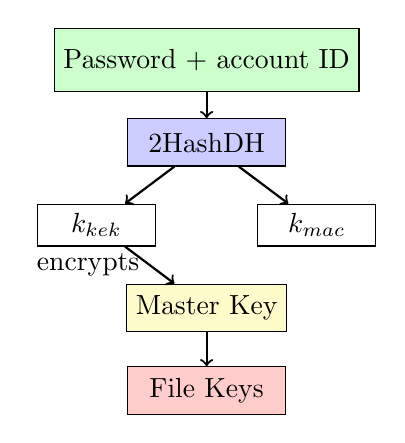
\begin{tikzpicture}[scale=0.7]
				% Password
				\node[draw, rectangle, minimum width=2.5cm, minimum height=0.8cm, fill=green!20] (password) at (0,5) {Password + account ID};

				% OPRF
				\node[draw, rectangle, minimum width=2cm, minimum height=0.6cm, fill=blue!20] (oprf) at (0,3.5) {2HashDH};
				\draw[->, thick] (password) -- (oprf);

				% Derived keys
				\node[draw, rectangle, minimum width=1.5cm, minimum height=0.5cm] (kkek) at (-2,2) {$k_{kek}$};
				\node[draw, rectangle, minimum width=1.5cm, minimum height=0.5cm] (kmac) at (2,2) {$k_{mac}$};
				\draw[->, thick] (oprf) -- (kkek);
				\draw[->, thick] (oprf) -- (kmac);

				% Master key
				\node[draw, rectangle, minimum width=2cm, minimum height=0.6cm, fill=yellow!20] (master) at (0,0.5) {Master Key};
				\draw[->, thick] (kkek) -- (master) node[midway, left] {encrypts};

				% File keys
				\node[draw, rectangle, minimum width=2cm, minimum height=0.6cm, fill=red!20] (filekeys) at (0,-1) {File Keys};
				\draw[->, thick] (master) -- (filekeys);
			\end{tikzpicture}
		\end{column}
	\end{columns}
\end{frame}

\begin{frame}{Registration and authentication flow}
	\begin{columns}[c]
		\begin{column}{0.5\textwidth}
			\textbf{Registration:}
			\begin{enumerate}
				\item Client samples OPRF key $k$, has account ID ($aid$)
				\item Computes $rw = \func{oprf}{aid, pw}$
				\item Derives $k_{kek}$, $k_{mac}$ from $rw$
				\item Generates random master key
				\item Encrypts master key with $k_{kek}$
				\item Sends to server: aid, $k$, $k_{mac}$, encrypted master key
			\end{enumerate}
		\end{column}
		\begin{column}{0.5\textwidth}
			\textbf{Authentication:}
			\begin{enumerate}
				\item Client initiates OPRF with server
				\item Server sends session ID (sid)
				\item Client recovers $rw$, derives keys
				\item Client MACs transcript with $k_{mac}$
				\item Server verifies MAC
				\item Server returns encrypted master key
				\item Client decrypts master key
			\end{enumerate}
		\end{column}
	\end{columns}
\end{frame}

\begin{frame}{File operations: Simple and secure}
	\begin{columns}[c]
		\begin{column}{0.5\textwidth}
			\textbf{Upload (put):}
			\begin{itemize}
				\item Generate random file key
				\item AEAD-encrypt file with file key
				\item AEAD-encrypt file key with master key
				\item Store header (encrypted file key)
				\item Store encrypted file content
			\end{itemize}
		\end{column}
		\begin{column}{0.5\textwidth}
			\textbf{Download (get):}
			\begin{itemize}
				\item Fetch encrypted header
				\item Decrypt file key with master key
				\item Fetch encrypted file
				\item Decrypt file with file key
				\item All bound to file ID via AEAD
			\end{itemize}
		\end{column}
	\end{columns}
	\vspace{0.5cm}
	\begin{center}
		Separate headers from content enables efficient sharing!
	\end{center}
\end{frame}

\begin{frame}{Sharing design: Each owner has their own header}
	\begin{columns}[c]
		\begin{column}{0.6\textwidth}
			\begin{itemize}
				\item \textbf{Sharing process:}
				      \begin{enumerate}
					      \item Owner fetches file key
					      \item Shares key out-of-band
					      \item Server adds new owner
					      \item Recipient wraps key under their master key
				      \end{enumerate}
				\item \textbf{Benefits:}
				      \begin{itemize}
					      \item No re-encryption on updates
					      \item Independent key management
					      \item Efficient for large files
					      \item Password changes don't affect shares
				      \end{itemize}
			\end{itemize}
		\end{column}
		\begin{column}{0.4\textwidth}
			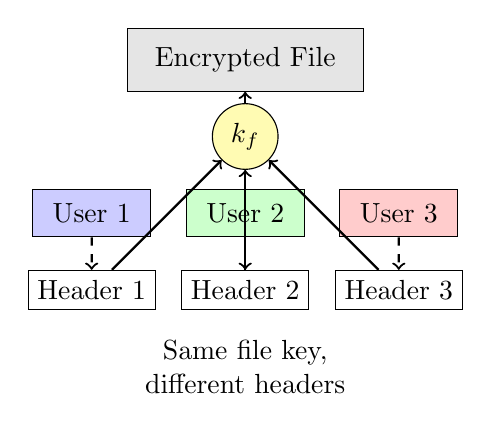
\begin{tikzpicture}[scale=0.65]
				% File
				\node[draw, rectangle, minimum width=3cm, minimum height=0.8cm, fill=gray!20] (file) at (0,3) {Encrypted File};

				% File key
				\node[draw, circle, fill=yellow!30] (filekey) at (0,1.5) {$k_f$};

				% Users
				\node[draw, rectangle, minimum width=1.5cm, minimum height=0.6cm, fill=blue!20] (user1) at (-3,0) {User 1};
				\node[draw, rectangle, minimum width=1.5cm, minimum height=0.6cm, fill=green!20] (user2) at (0,0) {User 2};
				\node[draw, rectangle, minimum width=1.5cm, minimum height=0.6cm, fill=red!20] (user3) at (3,0) {User 3};

				% Headers
				\node[draw, rectangle, minimum width=1.2cm, minimum height=0.5cm] (h1) at (-3,-1.5) {Header 1};
				\node[draw, rectangle, minimum width=1.2cm, minimum height=0.5cm] (h2) at (0,-1.5) {Header 2};
				\node[draw, rectangle, minimum width=1.2cm, minimum height=0.5cm] (h3) at (3,-1.5) {Header 3};

				% Connections
				\draw[->, thick] (filekey) -- (file);
				\draw[->, thick, dashed] (user1) -- (h1);
				\draw[->, thick, dashed] (user2) -- (h2);
				\draw[->, thick, dashed] (user3) -- (h3);
				\draw[->, thick] (h1) -- (filekey);
				\draw[->, thick] (h2) -- (filekey);
				\draw[->, thick] (h3) -- (filekey);

				\node[text width=3cm, align=center] at (0,-3) {Same file key, different headers};
			\end{tikzpicture}
		\end{column}
	\end{columns}
\end{frame}

\begin{frame}{Security properties achieved}
	\begin{columns}[c]
		\begin{column}{0.5\textwidth}
			\textbf{Against malicious server:}
			\begin{itemize}
				\item[\textcolor{green}{\mycheckmark}] No offline password attacks (OPRF)
				\item[\textcolor{green}{\mycheckmark}] Authenticated encryption throughout
				\item[\textcolor{green}{\mycheckmark}] Unique account ID prevents correlation
			\end{itemize}
		\end{column}
		\begin{column}{0.5\textwidth}
			\textbf{Design advantages:}
			\begin{itemize}
				\item[\textcolor{green}{\mycheckmark}] Password changes without re-encryption
				\item[\textcolor{green}{\mycheckmark}] Efficient file sharing
				\item[\textcolor{green}{\mycheckmark}] Simple, analyzable design
				\item[\textcolor{green}{\mycheckmark}] Uses only standard primitives
			\end{itemize}
		\end{column}
	\end{columns}
	\vspace{0.5cm}
	\begin{center}
		\textbf{This scheme has formal security proofs!}
	\end{center}
\end{frame}

\begin{frame}{Comparing with MEGA/Nextcloud}
	\begin{columns}[c]
		\begin{column}{0.33\textwidth}
			\textbf{MEGA}
			\begin{itemize}
				\item[\textcolor{red}{$\times$}] Custom crypto
				\item[\textcolor{red}{$\times$}] No AEAD
				\item[\textcolor{red}{$\times$}] Complex design
				\item[\textcolor{red}{$\times$}] No formal analysis
			\end{itemize}
		\end{column}
		\begin{column}{0.33\textwidth}
			\textbf{Nextcloud}
			\begin{itemize}
				\item[\textcolor{red}{$\times$}] Missing authentication
				\item[\textcolor{red}{$\times$}] Implementation bugs
				\item[\textcolor{red}{$\times$}] Ad-hoc design
				\item[\textcolor{red}{$\times$}] Feature creep
			\end{itemize}
		\end{column}
		\begin{column}{0.34\textwidth}
			\textbf{This scheme}
			\begin{itemize}
				\item[\textcolor{green}{\mycheckmark}] Standard primitives
				\item[\textcolor{green}{\mycheckmark}] AEAD everywhere
				\item[\textcolor{green}{\mycheckmark}] Clean hierarchy
				\item[\textcolor{green}{\mycheckmark}] Formal proofs
			\end{itemize}
		\end{column}
	\end{columns}
	\vspace{0.5cm}
	\begin{center}
		\textit{Simplicity and formal analysis make the difference!}
	\end{center}
\end{frame}

\begin{frame}{Key takeaways}
	\begin{columns}[c]
		\begin{column}{0.5\textwidth}
			\begin{itemize}
				\item \textbf{End-to-end encryption is hard to get right}
				      \begin{itemize}
					      \item Even major companies make critical mistakes
					      \item Ad-hoc designs inevitably fail
					      \item Retrofitting security doesn't work
				      \end{itemize}
				\item \textbf{Use established cryptographic building blocks}
				      \begin{itemize}
					      \item Don't roll your own crypto
					      \item Understand what primitives actually guarantee
					      \item Simplicity beats cleverness
				      \end{itemize}
			\end{itemize}
		\end{column}
		\begin{column}{0.5\textwidth}
			\begin{itemize}
				\item \textbf{Formal analysis is essential}
				      \begin{itemize}
					      \item Catches subtle vulnerabilities
					      \item Provides clear security guarantees
					      \item Should be done \textit{before} deployment
				      \end{itemize}
				\item \textbf{Trust models matter}
				      \begin{itemize}
					      \item Be honest about what you're protecting against
					      \item Users need verifiable security, not promises
					      \item Transparency builds trust
				      \end{itemize}
			\end{itemize}
		\end{column}
	\end{columns}
\end{frame}

\begin{frame}{\textit{And remember...}}
	\begin{columns}[c]
		\begin{column}{0.5\textwidth}
			\begin{center}
				{\Large The best cryptographic protocol is one that's\\
					\textit{simple enough to understand} and \textit{proven to be secure}} \\
				\vspace{1cm}
				{\small\textit{``Complexity is the enemy of security''}}
			\end{center}
		\end{column}
		\begin{column}{0.5\textwidth}
			\imagewithcaption{spamton_sez.png}{}
		\end{column}
	\end{columns}
\end{frame}

\begin{frame}[plain]
	\titlepage
\end{frame}
\end{document}
